\documentclass[reqno]{amsart}
\usepackage{amscd, amssymb, amsmath, amsthm, mathabx, mathrsfs}
\usepackage{graphicx}
\usepackage[colorlinks=true,linkcolor=blue]{hyperref}
\usepackage[utf8]{inputenc}
\usepackage[T1]{fontenc}
\usepackage{textcomp}
%% for identity function 1:
\usepackage{bbm}
%%For category theory diagrams:
\usepackage{tikz-cd}
\usepackage{enumitem}
\usepackage{float}
\usepackage{adjustbox}
\usepackage{todonotes}

\usepackage{caption}
\usepackage{subcaption}

\usepackage[backend=biber]{biblatex}
\addbibresource{mcg.bib}




\setlength\parindent{0pt}

\pdfsuppresswarningpagegroup=1

\newtheorem{theorem}{Theorem}[section]
\newtheorem{lemma}[theorem]{Lemma}
\newtheorem{proposition}[theorem]{Proposition}
\newtheorem{corollary}[theorem]{Corollary}
\newtheorem{conjecture}[theorem]{Conjecture}

\theoremstyle{definition}
\newtheorem{definition}[theorem]{Definition}
\newtheorem{example}[theorem]{Example}
\newtheorem{exercise}[theorem]{Exercise}
\newtheorem{problem}[theorem]{Problem}
\newtheorem{question}[theorem]{Question}

\theoremstyle{remark}
\newtheorem*{remark}{Remark}
\newtheorem*{note}{Note}
\newtheorem*{solution}{Solution}



%Inequalities
\newcommand{\cycsum}{\sum_{\mathrm{cyc}}}
\newcommand{\symsum}{\sum_{\mathrm{sym}}}
\newcommand{\cycprod}{\prod_{\mathrm{cyc}}}
\newcommand{\symprod}{\prod_{\mathrm{sym}}}

%Linear Algebra

\DeclareMathOperator{\Span}{span}
\DeclareMathOperator{\Ima}{Im}
\DeclareMathOperator{\diag}{diag}
\DeclareMathOperator{\Ker}{Ker}
\DeclareMathOperator{\ob}{ob}
\DeclareMathOperator{\Hom}{Hom}
\DeclareMathOperator{\sk}{sk}
\DeclareMathOperator{\Vect}{Vect}
\DeclareMathOperator{\Set}{Set}
\DeclareMathOperator{\Group}{Group}
\DeclareMathOperator{\Ring}{Ring}
\DeclareMathOperator{\Ab}{Ab}
\DeclareMathOperator{\Top}{Top}
\DeclareMathOperator{\hTop}{hTop}
\DeclareMathOperator{\Htpy}{Htpy}
\DeclareMathOperator{\Cat}{Cat}
\DeclareMathOperator{\CAT}{CAT}
\DeclareMathOperator{\Cone}{Cone}
\DeclareMathOperator{\dom}{dom}
\DeclareMathOperator{\cod}{cod}
\DeclareMathOperator{\Aut}{Aut}
\DeclareMathOperator{\Mat}{Mat}
\DeclareMathOperator{\Fin}{Fin}
\DeclareMathOperator{\rel}{rel}
\DeclareMathOperator{\Int}{Int}
\DeclareMathOperator{\sgn}{sgn}
\DeclareMathOperator{\PSL}{PSL}
\DeclareMathOperator{\GL}{GL}
\DeclareMathOperator{\Supp}{Supp}
\DeclareMathOperator{\tr}{tr}

%Row operations
\newcommand{\elem}[1]{% elementary operations
\xrightarrow{\substack{#1}}%
}

\newcommand{\lelem}[1]{% elementary operations (left alignment)
\xrightarrow{\begin{subarray}{l}#1\end{subarray}}%
}

%SS
\DeclareMathOperator{\supp}{supp}
\DeclareMathOperator{\Var}{Var}

%NT
\DeclareMathOperator{\ord}{ord}

%Alg
\DeclareMathOperator{\Rad}{Rad}
\DeclareMathOperator{\Jac}{Jac}

%Misc
\newcommand{\SL}{{\mathrm{SL}}}
\newcommand{\mobgp}{{\mathrm{PSL}_2(\mathbb{C})}}
\newcommand{\id}{{\mathrm{id}}}
\newcommand{\Mod}{{\mathrm{Mod}}}
\newcommand{\SMod}{{\mathrm{SMod}}}
\newcommand{\PMod}{{\mathrm{PMod}}}
\newcommand{\ud}{{\mathrm{d}}}
\newcommand{\Vol}{{\mathrm{Vol}}}
\newcommand{\Area}{{\mathrm{Area}}}
\newcommand{\diam}{{\mathrm{diam}}}
\newcommand{\Homeo}{{\mathrm{Homeo}}}
\newcommand{\SHomeo}{{\mathrm{SHomeo}}}


\newcommand{\reg}{{\mathtt{reg}}}
\newcommand{\geo}{{\mathtt{geo}}}

\newcommand{\tori}{{\mathcal{T}}}
\newcommand{\cpn}{{\mathtt{c}}}
\newcommand{\pat}{{\mathtt{p}}}

\let\Cap\undefined
\newcommand{\Cap}{{\mathcal{C}}ap}
\newcommand{\Push}{{\mathcal{P}}ush}
\newcommand{\Forget}{{\mathcal{F}}orget}
\newcommand{\Mon}{{\mathcal{M}}on}
\newcommand{\BMon}{{\mathcal{B}\mathcal{M}}on}



\title{Mapping Class Groups, Braid Groups and Geometric Representations}


\author{Jonas Trepiakas}



\begin{document}

\maketitle

\tableofcontents

\section{For the University of Bonn}


    This is a highly shortened version of the thesis which is
    originally 52 pages long. I have chosen the part which
    concerns the categorical framework into which geometric
    representations of braid groups can be put. In particular,
    my problem and goal in this thesis was to determine whether
    all the geometric representations in \cite{StSz} arise
    via Proposition \ref{yang-baxter-inducing-representation}
    on a suitably chosen monoidal category and 
    Yang-Baxter operator. The conclusion is that they indeed
    all arise in such a fashion. In particular, we show
    that the Birman-Hilden embedding can also be obtained
    from a Yang-Baxter operator in the category of decorated
    surfaces whereas it is usually obtained in the
    category of bidecorated surfaces.

\section{Introduction}


In this thesis, we develop the theory of mapping class groups
of surfaces and its connection to braid groups.

The goal of this thesis is to study connections
between these groups. In particular, we study
geometric representations which are homomorphisms
from braid groups into the mapping class group of some surface.

Our goal is to place these representations in
the more general categorical framework of monoidal categories
- primarily
following Harr, Vistrup and Wahl \cite{Harr-Vistrup-Wahl} and
Wahl and Randal-Williams \cite{Wahl-Randal-Williams}
where many representations are induced by so called Yang-Baxter
operators on certain monoidal categories of surfaces.

Using a classification of geometric representations
of braid groups on non-orientable surfaces by 
Stukow and Szepietowski \cite{StSz}, we show that
each such geometric representation is obtained 
by an appropriate choice of monoidal category of surfaces
and choice of Yang-Baxter operator - leaving certain cases
out.






\subsection{Thesis Summary} 

We show that
general monoidal categories that come equipped with a
so called Yang-Baxter element induce a geometric representation
of the braid group. We construct certain categories
of surfaces with Yang-Baxter elements which induce 
different geometric representations of the braid group, amongst
which we recover the Birman-Hilden embedding.\\

We then turn our attention to
geometric representations of the braid group on non-orientable
surfaces and once again recover previously constructed
representations in a new light. 





   \section{Braided monoidal categories}


\subsection{Yang-Baxter operators}



\begin{definition}[Yang-Baxter operator]
    Let $T \colon \mathcal{A} \to 
    \mathcal{V}$ be a functor from a category
    $\mathcal{A}$ to a monoidal category
    $\mathcal{V}$.
    A \textit{Yang-Baxter operator on $T$} is a natural family
    of isomorphisms
    \[
    y = y_{A,B} \colon
    T A \otimes TB \stackrel{\sim}{\to } TB \otimes TA
    \] 
    such that the following diagram commutes.

    \[\begin{tikzcd}\label{AA}
	{(TA \otimes TB) \otimes TC} & {TA \otimes(TB \otimes TC)} & {TA \otimes (TC \otimes TB)} & {(TA \otimes TC) \otimes TB} \\
	{(TB \otimes TA) \otimes TC} &&& {(TC \otimes TA) \otimes TB} \\
	{TB \otimes (TA \otimes TC)} &&& {TC \otimes (TA \otimes TB)} \\
	{TB \otimes (TC \otimes TA)} & {(TB \otimes TC) \otimes TA} & {(TC \otimes TB) \otimes TA} & {TC \otimes (TB \otimes TA)}
	\arrow["a", from=1-1, to=1-2]
	\arrow["{y \otimes TC}"', from=1-1, to=2-1]
	\arrow["{TA \otimes y}", from=1-2, to=1-3]
	\arrow["{a^{-1}}", from=1-3, to=1-4]
	\arrow["{y \otimes TB}", from=1-4, to=2-4]
	\arrow["a"', from=2-1, to=3-1]
	\arrow["a", from=2-4, to=3-4]
	\arrow["{TB \otimes y}"', from=3-1, to=4-1]
	\arrow["{TC \otimes y}", from=3-4, to=4-4]
	\arrow["{a^{-1}}"', from=4-1, to=4-2]
	\arrow["{y \otimes TA}"', from=4-2, to=4-3]
	\arrow["a"', from=4-3, to=4-4]
\end{tikzcd}\]

\end{definition}

\begin{remark}[]
    When $\mathcal{A} = \mathbbm{1}$, we say that
    $y$ is a Yang-Baxter operator on
    $X = T(\mathcal{A}) \in \mathcal{V}$ if
    it is a Yang-Baxter operator on 
    $T \colon \mathbbm{1} = \mathcal{A} \to 
    \mathcal{V}$.
\end{remark}


    Let $\left( \mathcal{X}, \otimes, I \right) $ be a
    monoidal category with $\tau \in 
    \Aut_{\mathcal{X}} \left( X \otimes X \right) $ 
    a Yang-Baxter operator in
    $\mathcal{X}$. Suppose
    $\mathcal{X}$ acts on a category
    $\mathcal{M}$ via a functor
    $\mathcal{M} \times \mathcal{X} \to \mathcal{M}$ 
    which we also denote by $\otimes$. Then 
    there is an action of the braid groupoid
     $\alpha_\tau \colon \mathcal{M} \times B \to 
     \mathcal{M}$ given on objects
     by
     $\alpha_{\tau} (A,n) = 
     A \otimes X^{\otimes n}$ and determined on morphisms
     by
     $\alpha_{\tau} \left( f, \sigma_i \right) 
     = f \otimes \id_{X^{\otimes i-1}} 
     \otimes \tau \otimes \id_{X^{\otimes n - i -1}}$.

     \begin{example}[]
         If $\mathcal{X} = \left( 
         \mathcal{X, \otimes, I}\right) $ admits a braiding
         $b$, then $\tau = b_{X,X} \in 
         \Aut_{\mathcal{X}} \left( X \otimes X \right) $ 
         is a Yang-Baxter operator for any object
         $X$. The thing that needs verifying here
         is that the big Yang-Baxter diagram in definition~\ref{AA}
         is satisfied, but
         this follows directly from
         proposition~\ref{braiding-gives-yang-baxter}.

         Likewise, for any functor
         $T \colon \mathcal{A} \to \mathcal{V}$ into a 
         braided tensor category $\mathcal{V}$, we obtain
         a Yang-Baxter operator as
         \[
         y_{A,B} = c_{TA,TB} \colon TA \otimes TB
         \stackrel{\sim}{\to } TB \otimes TA.
         \] 
         In particular, we obtain a Yang-Baxter operator
         on the inclusion functor 
         $\iota \colon \mathbbm{1} \to \mathcal{B}$ 
         identifying $\mathbbm{1}$ with the braid
         of a single string. We will
         denote this Yang-Baxter operator by $z$.
     \end{example}


     We want to show that the category of strong
     monoidal functors from the braid groupoid
     into $\mathcal{X}$ is equivalent to a naturally
     defined category of Yang-Baxter operators in
     $\mathcal{X}$.


     \begin{proposition}[]\label{yang-baxter-inducing-representation}
         For any strict monoidal category $\mathcal{V}$ and
         any Yang-Baxter $\tau$ on an element $X \in V$, there
         exists a unique strict monoidal functor
         $\Phi_{X, \tau} \colon \mathcal{B} \to \mathcal{V}$ such that
         $\Phi_{X, \tau} \circ z = y$.
     \end{proposition}


     \begin{proof}[Proof and construction]
         Define $\Phi_{X, \tau} \colon \mathcal{B} \to \mathcal{V}$ 
         on objects by $\Phi_{X,\tau} (n) = 
         X^{\otimes n}$. For
         $0 \le i < n$, define 
         \[
         y_i = X^{\otimes (i-1)} \otimes y 
         \otimes X^{\otimes (n-i-1)} \colon X^{\otimes n} \to 
         X^{\otimes n}.
         \] 
         These satisfy the braid group relations.
         Thus we obtain a monoid homomorphism
         $\Phi_{X, \tau, n} \colon \mathcal{B}_n \to 
         \mathcal{V} \left( X^{\otimes n}, X^{\otimes n} \right) $ 
         taking $\sigma_i$ to $y_i$ for all
         $0 \le i <n$. Clearly $\Phi_{X, \tau}$ is the unique
         strict monoidal functor with these properties.
     \end{proof}

     \begin{remark}[]
         In particular,
         $\Phi_{X,\tau,n} \colon
         \mathcal{B}_n \to \Aut_{\mathcal{V}}
         \left( X^{\otimes n} \right) $ for all
         $n$.\\

         As we said in the beginning, our goal
         is to get geometric representations from
         Yang-Baxter operators, so given our construction
         of $\Phi_{X,\tau}$, we might hope to
         find a category $\mathcal{V}$ such that
         its objects are surfaces and
         $\Aut_{\mathcal{V}} \left( X^{\otimes n} \right) $ 
         might correspond to a mapping class group. Indeed,
         this is what we shall do now in two
         different cases: the category of decorated surfaces
         and the category of bidecorated surfaces.
     \end{remark}




   \subsection{Braided monoidal category of decorated and
   bidecorated surfaces}

   \begin{definition}[Decorated surface]
       A decorated surface is a pair
       $(S,I)$ where $S$ is a compact connected
       surface with at least one boundary component
       and $I \colon \left[ -1,1 \right] 
       \hookrightarrow \partial S$ is a parametrised interval
       in its boundary.
   \end{definition}

   \begin{definition}[$\mathcal{M}_1$]
       Let $\mathcal{M}_1$ denote the groupoid where
       the objects are
       decorated surfaces and
       morphisms are isotopy classes of diffeomorphisms/homeomorphisms
       restricting to the identity on a neighborhood
       of $I$.
   \end{definition}

   \begin{remark}[]
       In particular, $\Aut_{\mathcal{M}_1} 
       \left( S \right) = \Mod (S)$.
   \end{remark}

   We now construct a braided monoidal structure on
   $\mathcal{M}_1$ : given decorated surfaces
   $\left( S_1, I_1 \right) $ and
   $\left( S_2,I_2 \right) $, define
   $\left( S_1, I_1 \right) 
   \otimes \left( S_2, I_2 \right) 
   := \left( S_1 \natural S_2, I_1 \natural I_2 \right) $ to be
   the surface obtained by gluing
   $S_1$ and $S_2$ along the right half-interval
   $I_1^{+} \in \partial S_1$ and the
   left half-interval $I_2^{-} \in \partial S_2$, defining
   $I_1 \natural I_2 = I_1^{-} \cup I_2^{+}$.

   \begin{figure}[htpb]
       \centering
       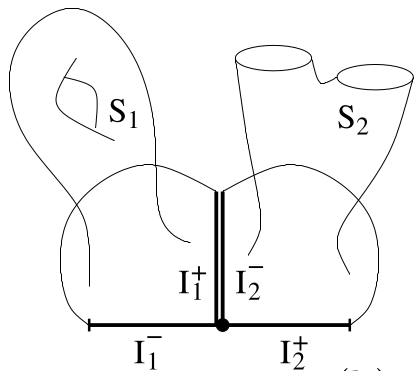
\includegraphics[width=0.35\textwidth]{connected-sum.png}
       \caption{$S_1 \# S_2$ \cite[Figure 2]{Wahl-Randal-Williams}}
       \label{fig:connected-sum-png}
   \end{figure}

   Furthermore, we define the unit object to be
   $I := \left( D^2, I \right) $. For it to be a strict unit, 
   we define $\left( S_1 \natural D^2, I_1 \natural I \right) 
   := \left( S_1, I_1 \right) $ and
   $\left( D^2 \natural S_2, I \natural I_2 \right) :=
   \left( S_2, I_2 \right) $.\\

   Note that this category is not strict as associativity 
   is not strict, but there is a way to construct an
   equivalent category which is strict \cite[Section
   3]{Galatius-Kupers-Randal-Williams}.\\
   

   We define a braiding $c$ on
   $\left( S_1 \natural S_2, I_1 \natural I_2 \right) $ 
   as the half-Dehn twist which satisfies that
   $c \colon \left( S_1 \natural S_2, I_1 \natural I_2 \right) 
   \stackrel{\sim}{\to } \left( S_2 \natural S_1, I_2 \natural I_1 \right)  $
   is a natural isomorphism because
   it has the opposite half-Dehn twist as the inverse. It is
   natural because the induced map will simply be the one induced by
   the naturality square.

   The B1 and B2 diagrams can be verified pictorially as follows:


   \begin{figure}[H]
    \centering
    \begin{minipage}[b]{0.7\textwidth}
        \centering
        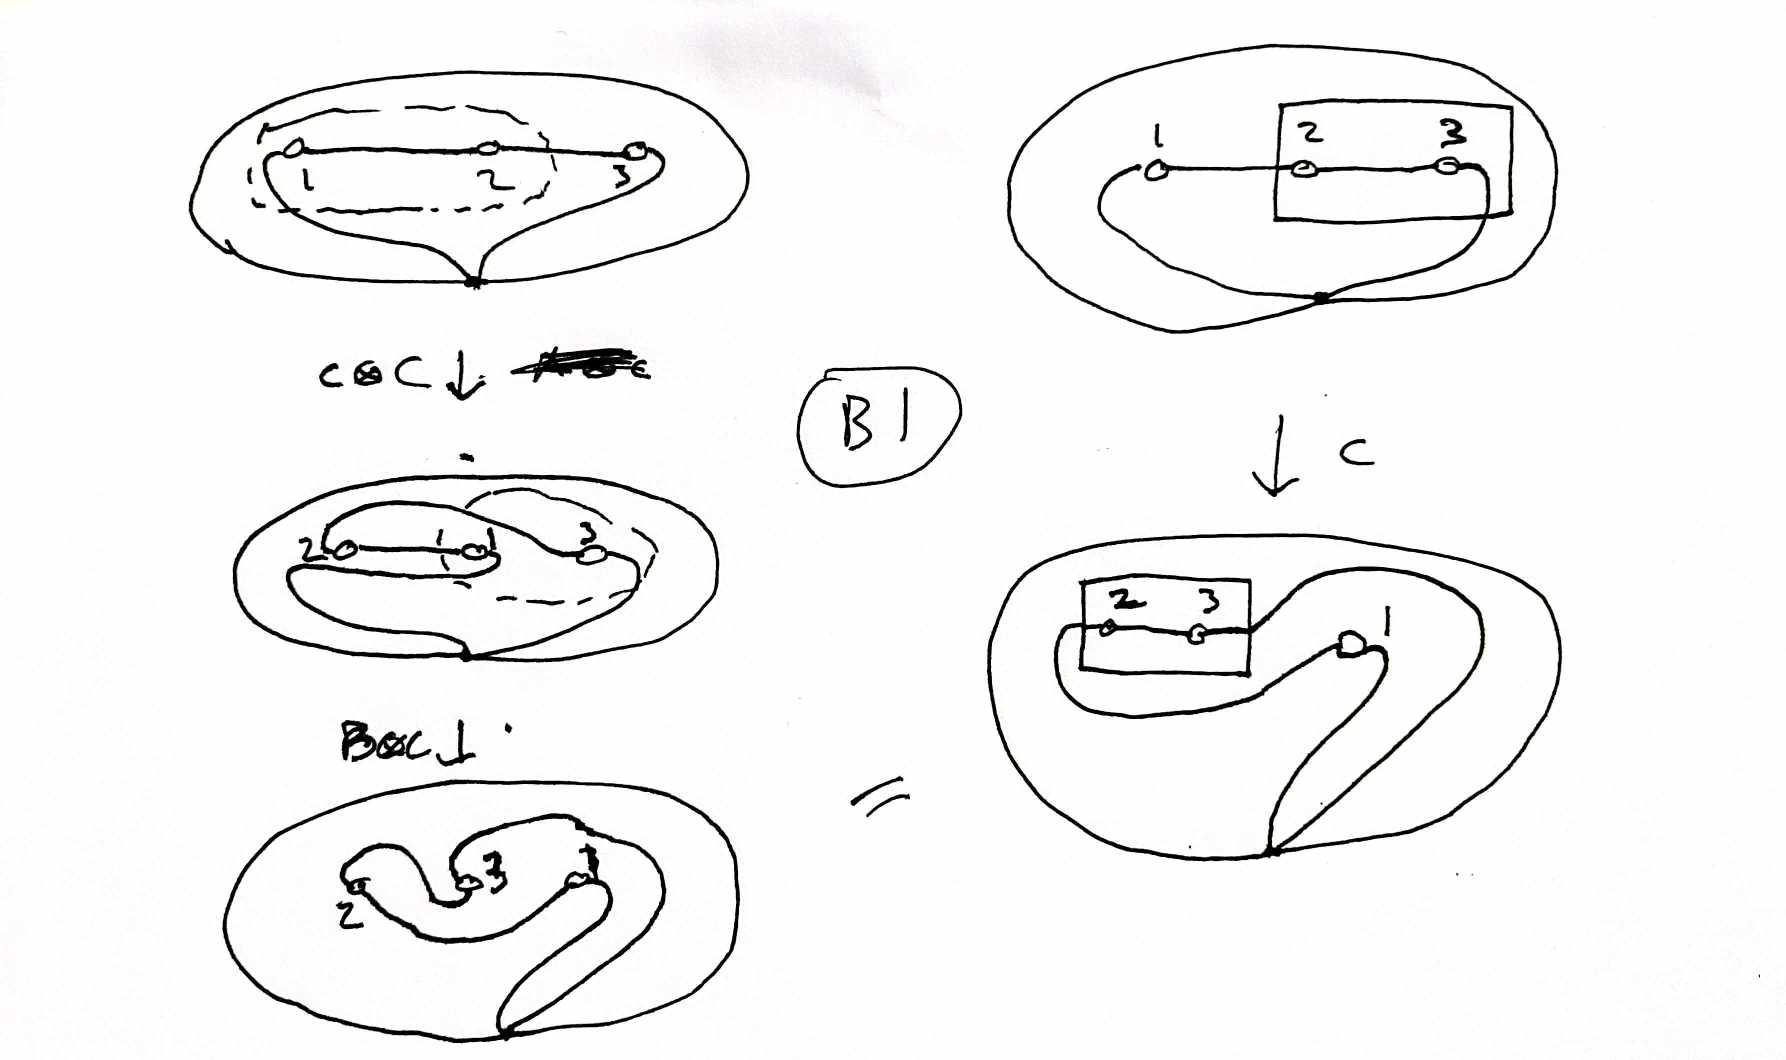
\includegraphics[width=1.1\textwidth]{B1.jpg} % first figure itself
    \end{minipage}\hfill
    \begin{minipage}[b]{0.7\textwidth}
        \centering
        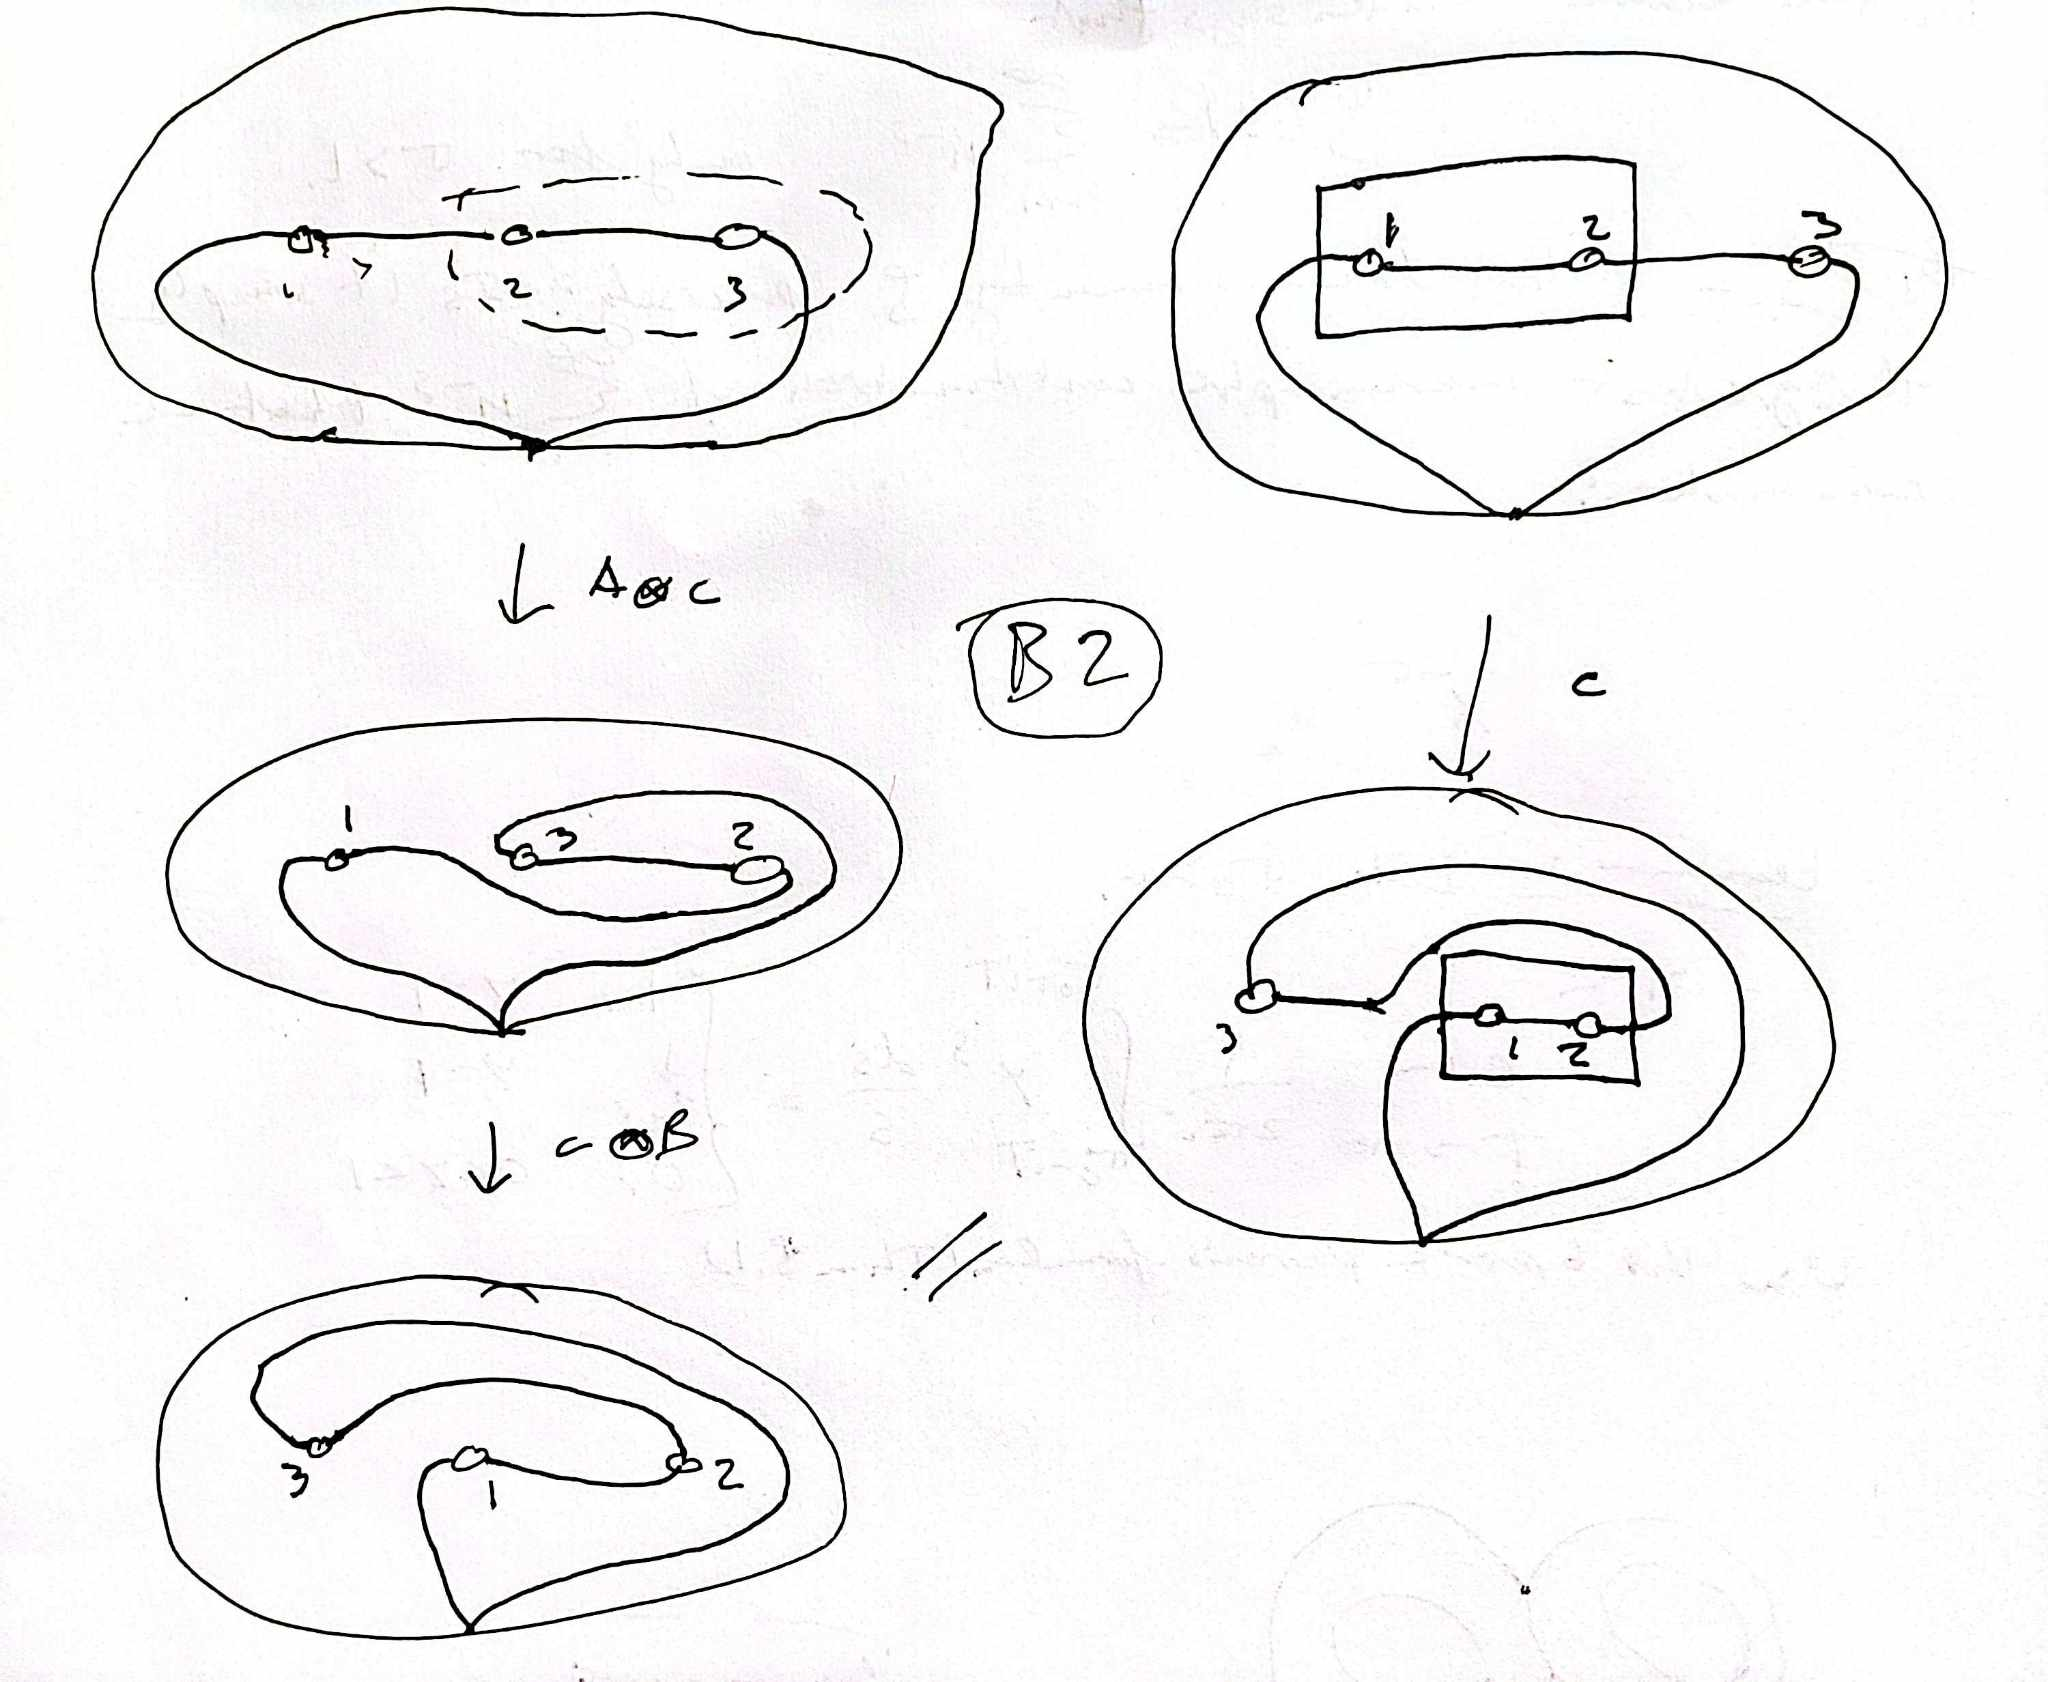
\includegraphics[width=0.9\textwidth]{B2.jpg} % second figure itself
    \end{minipage}
\end{figure}

This is precisely the requirements needed in
Proposition \ref{yang-baxter-inducing-representation}, so
we obtain a monoidal functor
$\Phi \colon \mathcal{B} \to \mathcal{M}_1$ 
such that $\Phi \circ z = y$ where
$y \in \Aut_{\mathcal{M}_1}
\left( S \natural S \right)
= \Mod \left( S \natural S \right) $
is the induced Yang-Baxter operator
on some decorated surface $S$ from the braiding.
So again, we obtain
a geometric representation
$\Phi_{n} \colon \mathcal{B}_n \to 
\Mod \left( S^{\natural n} \right) $\\
\linebreak


We will also consider a different monoidal category of
surfaces. Informally, a bidecorated surface is a surface with two 
intervals marked in its boundary.


    To give a precise definition, we first
    define certain surfaces $X_i$ that will be convenient for
    the monoidal structure, we set
    $X_1 = D^2 \subset \mathbb{C}$ to be the unit disk,
    and then define embeddings
    $\iota_1^{0}, \iota_1^{1} \colon I \to X_1$ by

    \[
    \iota_1^{0} (t) =
    e^{i \left( \frac{\pi}{4} + t \frac{\pi}{2} \right) }
    \quad
    \text{and}
    \quad
    \iota_{1}^{1} (t) = e^{i \left( 5 \frac{\pi}{4} +
    t \frac{\pi}{2} \right) }.
    \] 
    We denote by
    $\overline{\iota_1^{i}} \colon
    I \to X_1$ the reverse map
    $t \mapsto \iota_{1}^{i}(1-t)$ for $i = 0,1$.
    Then we recursively define $X_{m+1}$ for 
    $m\ge 1$ by
    \[
    X_{m+1} :=
    \frac{X_m \sqcup X_1}{\iota_m^{i}(t) 
\sim \overline{\iota_1^{i}}} \quad \text{for } t
\in \left[ \frac{1}{2},1 \right]
    \] 
    and we define
    \[
    \iota_{m+1}^{i} (t) 
    =
    \begin{cases}
        \iota_m^{i}(t),& \text{if } t \le \frac{1}{2}\\
        \iota_1^{i}(t),& \text{else}
    \end{cases}.
    \] 

    In this process, the marked intervals will live in
    different boundary components every second time. 
    The process for each of the two situations is illustrated below
    in figures
    \ref{fig:bidecorated-attaching-jpeg} and
    \ref{fig:bidecorated-second-attaching-jpeg}.


\begin{figure}[H]
    \centering
    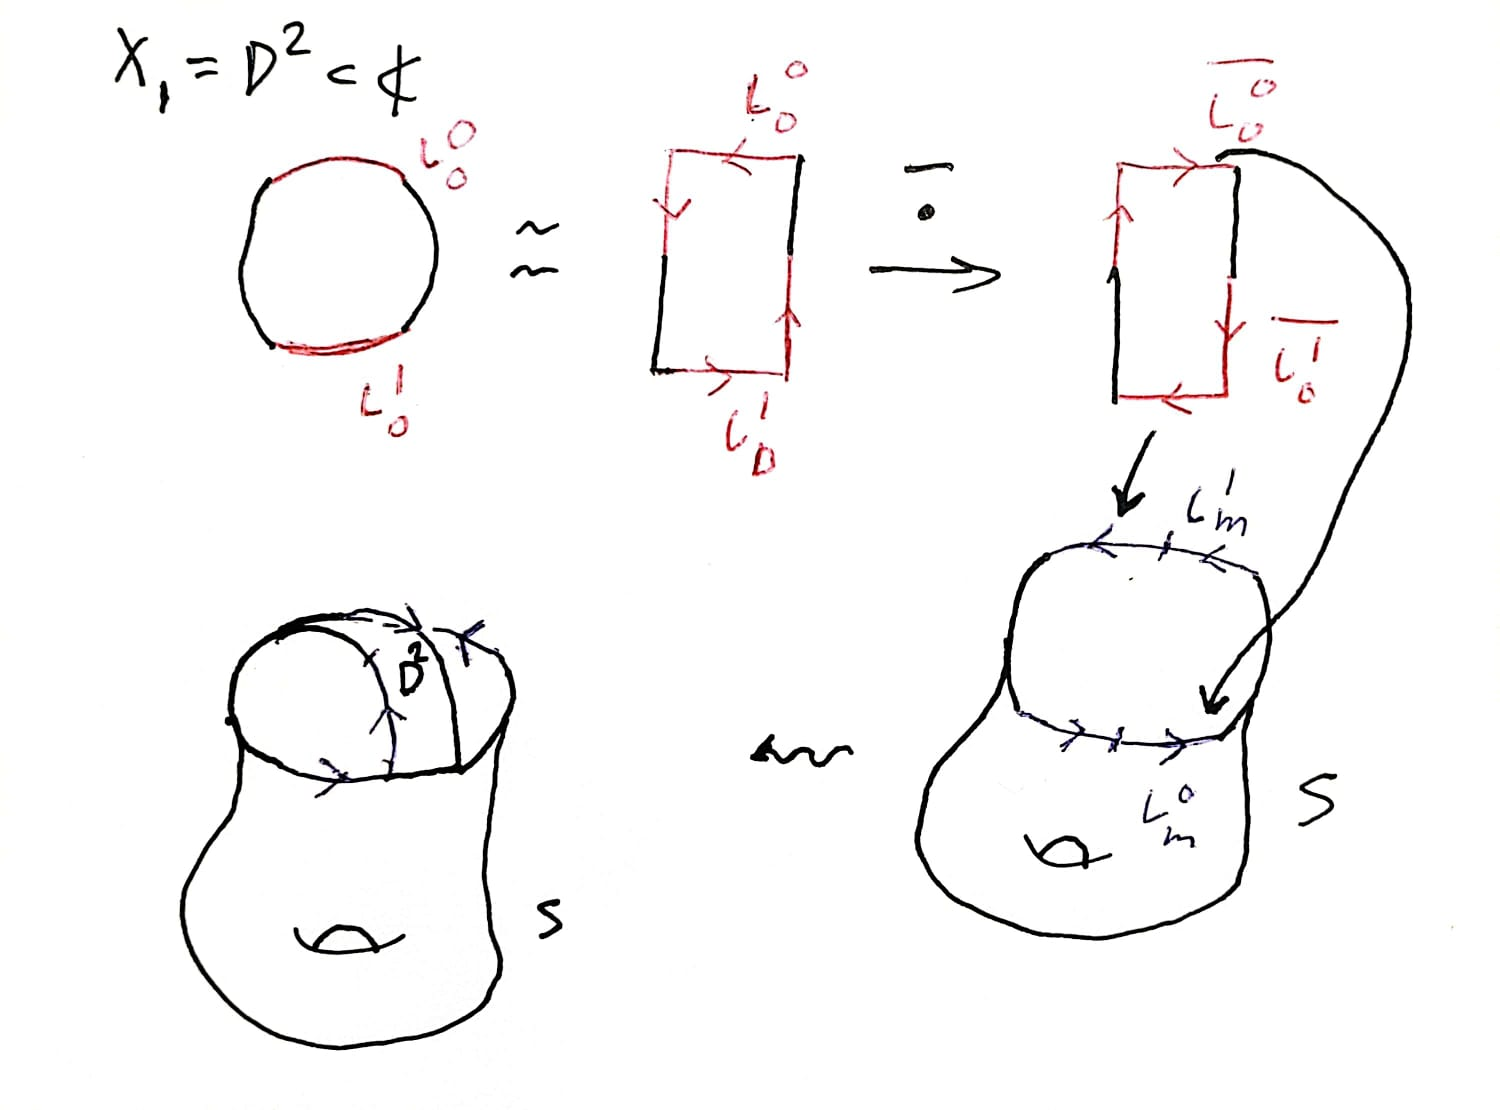
\includegraphics[width=0.6\textwidth]{bidecorated-attaching.jpeg}
    \caption{Marked intervals in single boundary components.}
    \label{fig:bidecorated-attaching-jpeg}
\end{figure}

\begin{figure}[H]
    \centering
    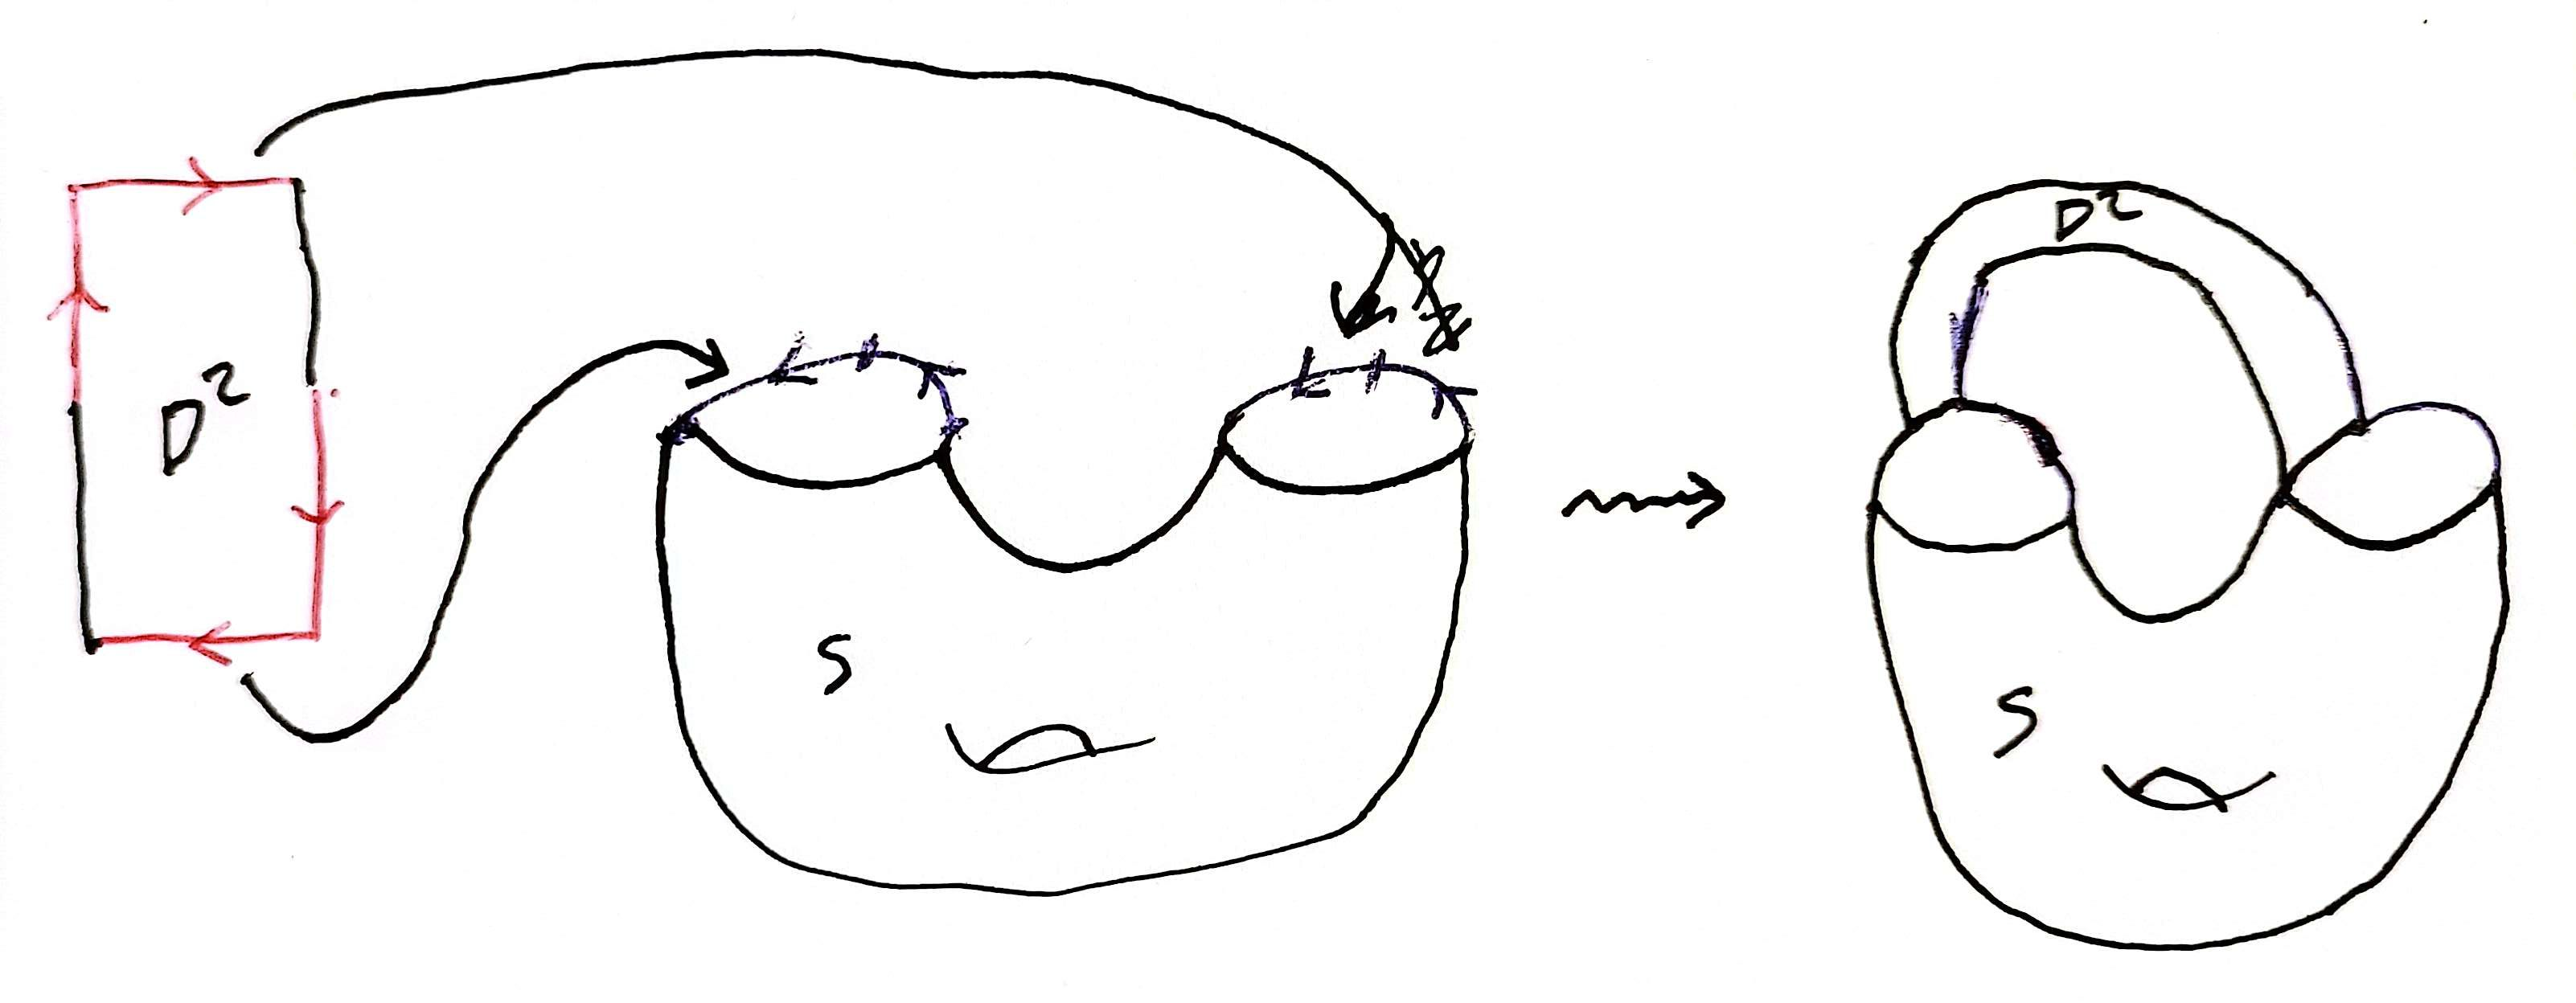
\includegraphics[width=0.6\textwidth]{bidecorated-second-attaching.jpeg}
    \caption{Marked intervals in different boundary components.}
    \label{fig:bidecorated-second-attaching-jpeg}
\end{figure}

\begin{lemma}[]
    For $m\ge 1$, $X_m \approx S_{g,r}$ where
    \[
        \left( g,r \right) =
        \begin{cases}
            \left( \frac{m}{2}-1,2 \right) ,& m \text{ even}\\
            \left( \frac{m-1}{2},1 \right) ,& m \text{ odd}
        \end{cases}.
    \] 
\end{lemma}

\begin{proof}
    Firstly, $X_m$ is clearly connected, and
    we have
    \[
    \chi \left( X_{m} \right) 
    = \chi \left( X_{m-1} \right) -1
    \] 
    since, for example, the $\Delta$-structure on
    our surface $X_{m}$ can be chosen to be that for $X_{m-1}$ with
    the boundary subdivided into four $2$-simplices with 
    four vertices,
    adding an additional two $2$-simplices and then
    a disk.
    By induction, we then get
    $\chi \left( X_{m} \right) 
    = \chi \left( X_1 \right) - \left( m-1 \right) 
    = 2-m$.\\
    Now, by the classification of surfaces with
    boundary and genus, we simply need to
    know how many boundary components $X_{m+1}$ has.
    But as can be seen from the figures, 
    if $m$ is odd, we will have one boundary component,
    while if  $m$ is even, we will have
    two boundary components.
\end{proof}

\begin{definition}[Bidecorated surface]
    A bidecorated surface is a tuple
    $\left( S, m , \varphi  \right) $ where
    $S$ is a surface, $m\ge 1$ is an integer,
    and
    \[
    \varphi \colon
    \partial X_m \sqcup \left( \sqcup_{k} S^{1} \right) 
    \stackrel{\sim}{\to } \partial S
    \] 
    is a homeomorphism, giving a parametrization of the boundary of
    $S$. We think of $\left( S, m , \varphi  \right) $ as
    a surface with two parametrized arcs
    \[
    I_0 := \varphi \circ \iota_{m}^{0} \quad
    \text{and} \quad 
    I_1 := \varphi \circ \iota_m^{1}
    \] 
    in its boundary, and $k$ additional parametrized
    boundaries.
\end{definition}


\begin{definition}[$\mathcal{M}_2$]
    Let $\mathcal{M}_2$ denote the monoidal groupoid
    where objects are bidecorated surfaces together
    with a formal unit $U$. The Hom set
    between two bidecorated surfaces
    $\left( S, m, \varphi  \right) $ and
    $\left( S', m', \varphi' \right) $ is
    empty if $m\neq m'$ or $S$ and $S'$ are nonhomeomorphic.
    Otherwise, the Hom set consists of all mapping
    classes of homeomorphisms that preserve the
    boundary parametrizations:
    \[
    \Hom_{\mathcal{M}_2}\left( 
    \left( S,m,\varphi  \right) , 
\left( S', m, \varphi' \right) \right) 
= 
    \pi_0 \Homeo_{\partial}\left( S,S' \right) 
    = \pi_0 \left\{ f \in \Homeo \left( S,S' \right) 
    \mid f \circ \varphi  = \varphi' \right\}
\] 
where $\Homeo\left( S,S' \right) $ has the compact-open
topology, and 
$\Homeo_{\partial}\left( S,S' \right) $ the subspace topology.
\end{definition}

\begin{remark}[]
    We again obtain that
    $\Aut_{\mathcal{M}_2}
    \left( \left( S,m,\varphi  \right)  \right) 
    = \Mod (S)$.
\end{remark}

The monoidal structure $\natural^2 $ on $\mathcal{M}_2$ is defined
as follows. The object $U$ is by definition a unit,
and for the remaining objects, we define
\[
    \left( S,m, \varphi  \right) \natural^2
    \left( S',m', \varphi ' \right) 
    :=
    \left( \frac{S \sqcup S'}{I_i(t)
    \sim \overline{I_i'}(t), t \in 
\left[ \frac{1}{2},1 \right] }, m+m',
\varphi \natural^2 \varphi ' \right) 
\] 
for $i = 0,1$, and where
\[
\varphi \natural^2 \varphi ' \colon
\partial X_{m+m'} \sqcup \left( \sqcup_{k+k'}
S^{1}\right) \hookrightarrow \partial
\left( S \natural^2 S' \right) 
\] 
is obtained using the canonical identification
$\partial X_{m+m'} \approx 
\left( \partial X_{n - \iota_m \left( \frac{1}{2},1
\right) } \right) \cup 
\left( \partial X_{m'} - 
\iota_{m'} \left( 0, \frac{1}{2} \right) \right)$.

Now we will construct a Yang-Baxter element
in $\mathcal{M}_2$ as follows. Let
$D^{\natural^2 m} = D_1 \natural^2 \ldots \natural^2
\left( D_i \natural^2 D_{i+1} \right) 
\natural^2 \ldots \natural^2 D_m$, where subscripts are used to enumerate
the disks. The underlying surface, by construction, will
be $X_m$. Let
$a_i$ denote the isotopy class of a curve in the interior
$D_i \natural^2 D_{i+1} \approx
S^{1} \times I$ that is parallel to its
boundary components, see figure \ref{fig:curve-m-2-png}.

\begin{figure}[H]
    \centering
    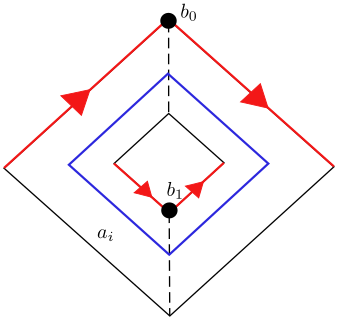
\includegraphics[width=0.4\textwidth]{curvem2.png}
    \caption{The curve $a_i$ in $D_i \natural D_{i+1}$
    \cite[Figure 4]{Harr-Vistrup-Wahl}}
    \label{fig:curve-m-2-png}
\end{figure}

\begin{lemma}[]
    The curves $a_1, \ldots, a_{m-1}$ form a chain in
    $D^{\natural^2 m}$.
\end{lemma}

\begin{proof}
    The curve $a_i$ has image contained in $D_i \natural^2 D_{i+1}$,
    so it can only intersect $a_{i-1}$ and $a_{i+1}$ nontrivially.
    So it suffices to look at the subsurface of
    $D^{\natural^2 m}$ corresponding to
    $D_i \natural^2 D_{i+1} \natural^2 D_{i+2}$.

    \begin{figure}[H]
        \centering
        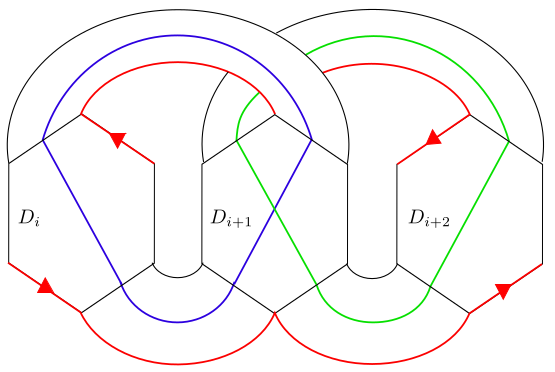
\includegraphics[width=0.6\textwidth]{intersection-a_is.png}
        \caption{Intersection of
        $a_i$ and $a_{i+1}$ in
    $D_i \natural^2 D_{i+1} \natural^2 D_{i+2}$.
\cite[Figure 5]{Harr-Vistrup-Wahl}}
        \label{fig:intersection-a_is-png}
    \end{figure}
\end{proof}


Now by Lemma \ref{dehn-intersection-0} and Proposition \ref{dehn-braid-relation}
(the braid relation), we get that the
braid group relations hold for the Dehn twists
$T_i \in \Aut_{\mathcal{M}_2}\left( D^{\natural^2 m} \right) $ 
where $T_i$ is the Dehn twist along the curve
$a_i$ in $D^{\natural^2 m}$, i.e.,
\begin{align*}
    T_{i}T_{i+1}T_i 
    &= T_{i+1} T_i T_{i+1} &\forall i\\
    T_i T_j 
    &= T_j T_i &\text{for } \left| i-j \right| >1
\end{align*}
Hence the same relations hold for the
inverses $T_{i}^{-1}$.\\
\linebreak
If we add a disk to either side of $D^{\natural^2 m}$, we get
\[
T_i \natural^2 \id_{D} = T_i \quad \text{and} \quad
\id_{D}\natural^2 T_i = T_{i+1}
\] 
in $\Aut_{\mathcal{M}_2}\left( D^{\natural^2 m+1} \right) $.
Hence this gives the relation
\[
    \left( T_1^{-1} \natural^2 \id_D \right) \left( \id_D \natural^2
    T_1^{-1} \right) \left( T_1^{-1} \natural^2 id_D \right) 
    = 
    \left( \id_D \natural^2 T_1^{-1} \right) 
    \left( T_1^{-1} \natural^2 \id_D \right) 
    \left( \id_D \natural^2 T_1^{-1} \right) 
\] 
in $\Aut_{\mathcal{M}_2} \left( D^{\natural^2 3} \right) $,
meaning that $T_1^{-1}$ is a Yang-Baxter element. This
yields a monoidal functor
\[
\Phi = \Phi_{D, T_1^{-1}} \colon
\left( \mathcal{B}, \otimes \right) 
\to \left( \mathcal{M}_2, \natural^2 \right) 
\] 
uniquely determined up to monoidal natural
isomorphism by
$\Phi (n) = D^{\natural^2 n}$ and
$\Phi_{D, T_1^{-1}, n} \left( \sigma_1 \right) =
D^{\natural^2 i-1} \natural^2  T_1^{-1} \natural^2
D^{\natural^2 n - i -1} =
T_i^{-1} \in 
\Aut_{\mathcal{M}_2}\left( D^{\natural^2 m} \right) 
= \pi_0 \Homeo_{\partial} \left( X_m \right)$.
Seeing that this is exactly
the setup for the Birman-Hilden theorem,
we note that the homomorphisms
\[
    \Phi_m = \Phi_{D,T_1^{-1},m}
\colon B_m \to \Aut_{\mathcal{M}_2}
\left( D^{\natural^2 m} \right) \approx
\Aut_{\mathcal{M}_2} \left( 
X_m\right)
\approx
\begin{cases}
    \Mod 
    \left( S_{\frac{m}{2}-1,2} \right) ,& m\text{ even}\\
    \Mod \left( 
S_{\frac{m-1}{2}, 1} \right),& m\text{ odd}
\end{cases}.
\] 
recover the Birman-Hilden embeddings from
section \ref{birman-hilden-embedding-construction}.
















\section{Geometric Representations of the Braid Group on
non-orientable surfaces}

We will now look at the classified geometric representations
of braid groups on non-orientable surfaces as presented
in \cite{StSz}. In particular, we will explore how the
representations fit in our categorical framework from the previous
section.\\

We start by noting some facts about non-orientable surfaces.\\
\linebreak


A connected orientable (respectively nonorientable) surface
of genus $g$ with $b$ boundary components will
be denoted by $S_{g,b}$ (respectively $N_{g,b}$ ).

Now, recall that the Möbius band (which is also called
a crosscap), is the mapping cylinder on the map
$z \mapsto z^2$ (see figure~\ref{fig:mapping-cylinder-mobius})
We will denote the Möbius band by $M$.


\begin{figure}[htpb]
    \centering
    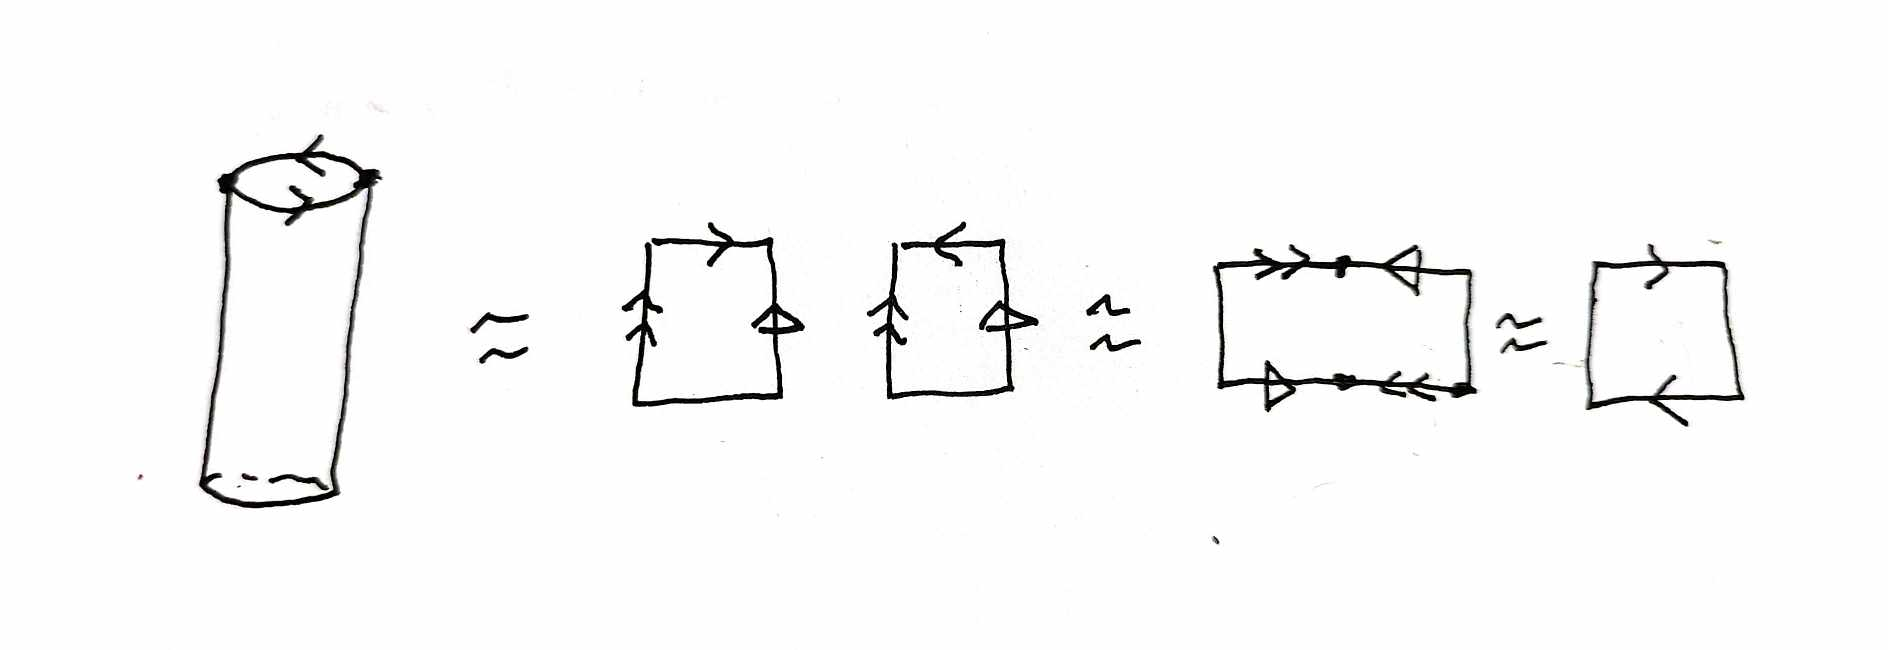
\includegraphics[width=0.7\textwidth]{mapping-cylinder-mobius.jpg}
    \caption{Möbius band}
    \label{fig:mapping-cylinder-mobius}
\end{figure}

In this case, any of the two curves making up the half-circles which
get identified can be cut along, rendering a connected surface.
Thus gluing on a Möbius strip along the boundary, we obtain a
surface of one higher genus.\\


We can then obtain $N_{g,b}$ from $S_{0,g+b}$ by
gluing $g$ Möbius bands along $g$ distinct boundary
components of $S_{0,g+b}$.

Note that by the classification of surfaces
\[
N_{g,b} \approx \left( \mathbb{R}\mathbb{P}^2 \right)^{\# g} -
\sqcup_{b} \mathring{D} \approx 
 \left(\mathbb{R}\mathbb{P}^2 - \mathring{D} 
\right)^{\natural g} - \sqcup_{b-1} \mathring{D}
\] 
where $\mathbb{R}\mathbb{P}^2 - \mathring{D}$ is a Möbius band.

Note also that $\mathbb{R}\mathbb{P}^2 \# \mathbb{R}\mathbb{P}^2
\approx K$, the Klein bottle,
see figure~\ref{fig:klein-bottle}.


\begin{figure}[H]
    \centering
    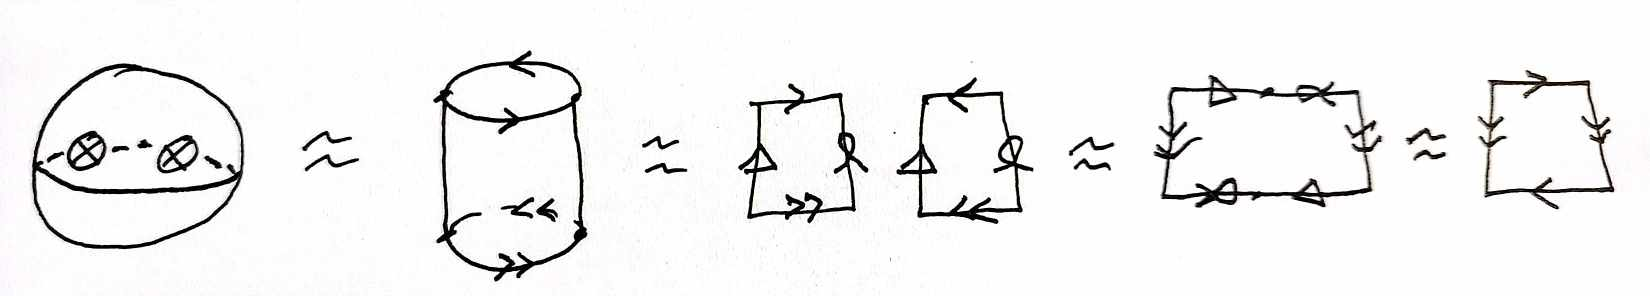
\includegraphics[width=1.2\textwidth]{klein-bottle.jpg}
    \caption{Klein-bottle as the sphere with two crosscaps}
    \label{fig:klein-bottle}
\end{figure}

\begin{lemma}[]\label{prop61}
    $N_{g,1} \approx S_{n,1} \natural M$ for
    $g = 2n+1$.
\end{lemma}

\begin{proof}

For $g = 2n+1$ with $n\ge 0$, we have
(see \ref{fig:N_3-1-jpg} for a visual argument for
$T^2 \# M \approx K \# M$ - 
to see why the top-right surface is $K - D^2$, take
the usual Klein-bottle, remove a disk such that
it is embeddable in $\mathbb{R}^{3}$, and
then enlarge the hole.)
\begin{align*}
N_{2n+1,1} \approx
\left( \mathbb{R}\mathbb{P}^2 \right)^{\# 2n+1} -
\mathring{D} 
&\approx K^{\# n} \# M
\approx K^{\# n-1} \# K \# M\\
&\approx K^{\# n-1} \# T^2 \# M\\
&\approx \ldots\\
&\approx \left( T^2 \right)^{\# n} \# M\\
&\approx S_{n,0} \# M\\
&\approx S_{n,1} \natural M
\end{align*}

\end{proof}


\begin{figure}[H]
    \centering
    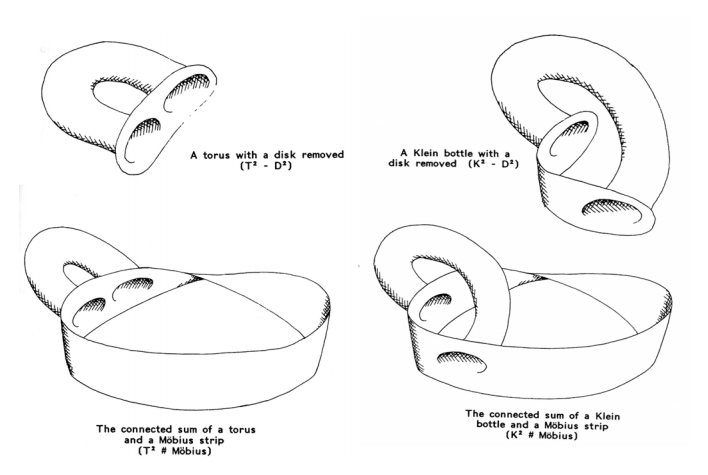
\includegraphics[width=1\textwidth]{N_3,1.jpg}
    \caption{A hemeomorphism between 
    $T^2 \# M$ and $K \# M$ \cite[Figure 5.7]{Weeks}}
    \label{fig:N_3-1-jpg}
\end{figure}





Hence for $g$ odd, we have an embedding
$B_{g} \hookrightarrow N_{g,1}$ by the Birman-Hilden
embedding into the $S_{n,1}$ summand. A similar thing
can be done for the even case.\\
\linebreak



We will now introduce different types of representations
of the braid group on non-orientable surfaces.


\begin{definition}[]
We call a curve two-sided (resp. one-sided) if its regular neighborhood is an
annulus (resp a Möbius band).
\end{definition}

\subsubsection{The standard twist representation}

\begin{lemma}[]
    Take a chain of two-sided curves
    $C = \left( a_1, \ldots, a_{n-1} \right) $.
    If we fix an orientation of a regular neighborhood
    of the union of the curves $a_i$, then
    $C$ determines \textit{the standard twist representation}
    $\rho_{C} \colon B_n \to \PMod (S)$ defined by
    \[
    \rho_C \left( \sigma_i \right) = t_{a_i}, \quad
    i = 1, \ldots, n-1,
    \] 
    where $t_{a_i}$ is the right-handed Dehn twist
    about $a_i$ with respect to the orientation.
\end{lemma}

\begin{figure}[H]
    \centering
    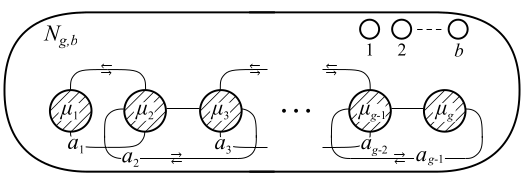
\includegraphics[width=0.8\textwidth]{standard-chain.png}
    \caption{Standard chain of non-separating curves
    in $N_{g,b}$ \cite[Figure 1]{StSz}}
    \label{fig:standard-chain-png}
\end{figure}

\begin{question}
    One might wonder whether the standard twist representation
    corresponds to an induced representation from a Yang-Baxter
    operator on some category of surfaces.
\end{question}

To answer this question, the intuitive monoidal category to
look at given Figure \ref{fig:standard-chain-png} is
$\mathcal{M}_1$ with a Yang-Baxter operator
on the Möbius band with the parametrized interval
as depicted on the left in Figure \ref{fig:mobius-decorated-jpg}
and the Yang-Baxter operator given by
the homeomorphism which is the Dehn twist about the curve in
$M \natural M$ depicted on the right side in Figure
\ref{fig:mobius-decorated-jpg}.

Continuing in this manner, we find that
$M^{\natural g}$ is as depicted in
Figure \ref{fig:Ng1-jpg} which is homeomorphic to
$N_{g,1}$, and we see that the loops precisely coincide with
those from the standard chain depicted in
Figure \ref{fig:standard-chain-png}.

Now, note that the Yang-Baxter equation in this case
again is satisfied because of the
braid relation for Dehn twists,
Proposition \ref{dehn-braid-relation}. Thus
we obtain a monoidal functor
$\Phi_{M, std} \colon \mathcal{B} \to 
\mathcal{M}_1$ with
$\Phi_{M, std, g} \colon \mathcal{B}_n
\to \Mod \left( N_{g,1} \right) $ the standard twist representation.

\begin{figure}[H]
    \centering
    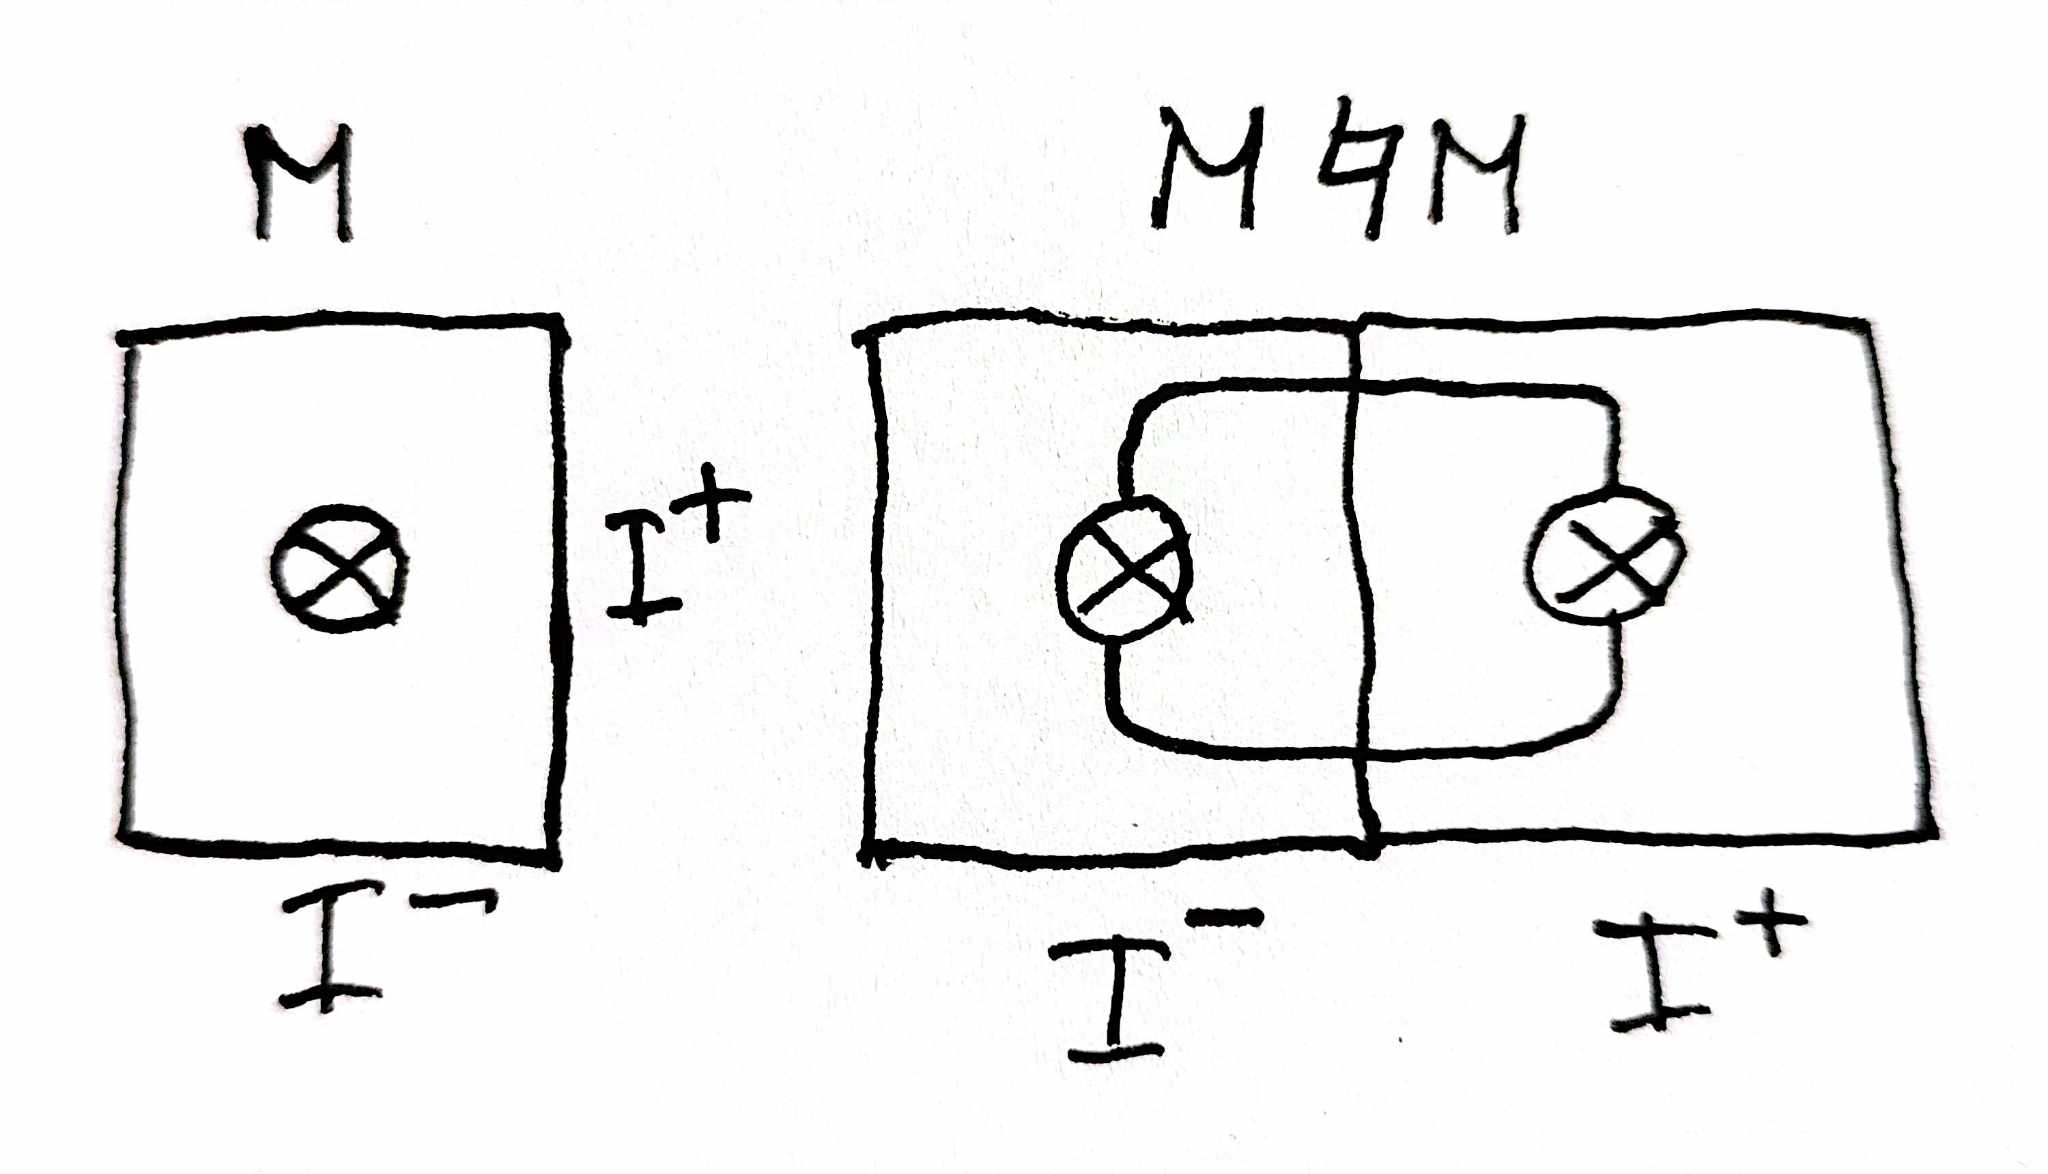
\includegraphics[width=0.4\textwidth]{mobius-decorated.jpg}
    \caption{mobius-decorated.jpg}
    \label{fig:mobius-decorated-jpg}
\end{figure}

\begin{figure}[H]
    \centering
    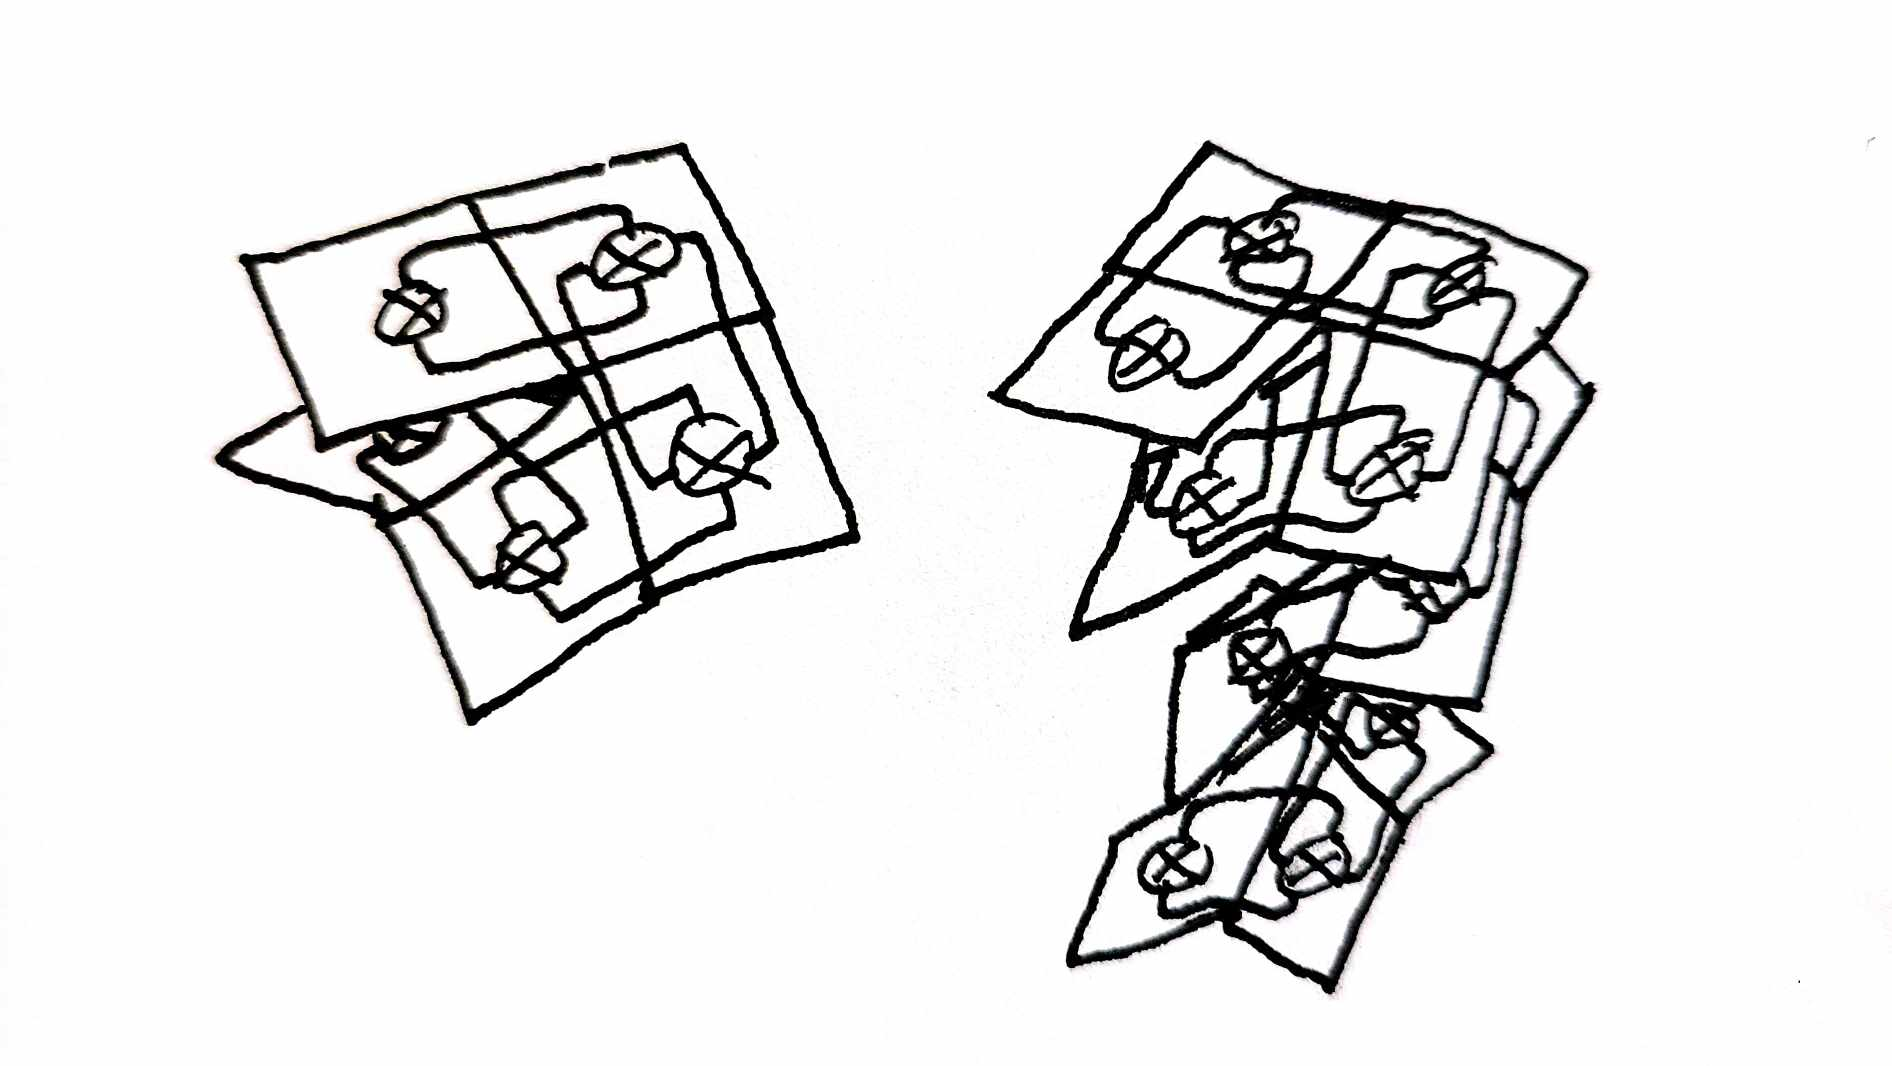
\includegraphics[width=0.8\textwidth]{Ng1.jpg}
    \caption{The standard chain in
    $M^{\natural g} \approx N_{g,1}$.}
    \label{fig:Ng1-jpg}
\end{figure}



Recall that the Birman-Hilden embedding was obtained
as an induced geometric representation from a Yang-Baxter
operator in the category of bidecorated surfaces.

The following proposition shows that 
the standard twist representation, in fact, 
is also the Birman-Hilden embedding now obtained
from a Yang-Baxter operator in the category of
decorated surfaces and in a seemingly different form.

\begin{proposition}[]\label{standard-twist-birman-hilden}
    For $b\ge 1$ and
    $g$ odd, the standard twist representation
    $\rho_{C} \colon B_g \to \Mod (N_{g,b})$ is the
    same as the Birman-Hilden embedding
    $B_g \hookrightarrow S_{\frac{g-1}{2}, b-1} \# M $
    into the orientable factor.
\end{proposition}

\begin{proof}

To make use of the visualization from Figure
\ref{fig:N_3-1-jpg}, we need the steps to go from 
$K - D^2$ as a sphere with two crosscaps and a disk removed
to the depiction in Figure \ref{fig:N_3-1-jpg}.

Suppose we look at the standard chain of non-separating curves
in $N_{3,b}$, so we have curves $a_1$ and $a_2$ as
in Figure \ref{fig:standard-chain-png}.
Now, since
 $N_{3,1} = K \# M $, we can decompose the loops
 $a_1$ and $a_2$ and follow
 it through the homeomorphisms for
 $K - D$ and for $M - D$ as in 
 in Figure \ref{fig:part1-deformation-curve-jpg} and
 Figure \ref{fig:part2-deformation-curve-jpg}.

 After the transformations, we reglue the surfaces
 and twist
 the tube from the Klein bottle around
 to obtain a torus 
 as in Figure \ref{fig:klein-to-torus-curve-jpg}.

 Now, noting that 
 \[
 N_{2g+1,b}
 \approx 
 \left( \left( \mathbb{R}\mathbb{P}^2 - \mathring{D} \right)
\natural \left( \mathbb{R}\mathbb{P}^2 
- \mathring{D} \right)\right)^{\natural g}
\natural M - \bigsqcup_{b-1} \mathring{D} 
= K^{\natural g} \natural M - 
\bigsqcup_{b-1} \mathring{D}
= \left( K^{\natural g} \right) 
\]
we find that for $N_{2g+1,1}$ with $g>1$, we get a similar
picture as for $N_{3,1}$, depicted in Figure
\ref{fig:many-klein-torus-curve-jpg}, where
we can also twist the tube around.

In conclusion, the loops really correspond to a
standard chain in $S_g$, so the
standard twist representation
$\rho_{C} \colon
B_{2g+1} \to \Mod \left( N_{2g+1,1} \right) 
\approx \Mod \left( S_{g,1} \natural M \right) $ 
corresponds to the Birman-Hilden embedding
into the $S_{g,1}$ factor.



\begin{figure}[htpb]
    \centering
    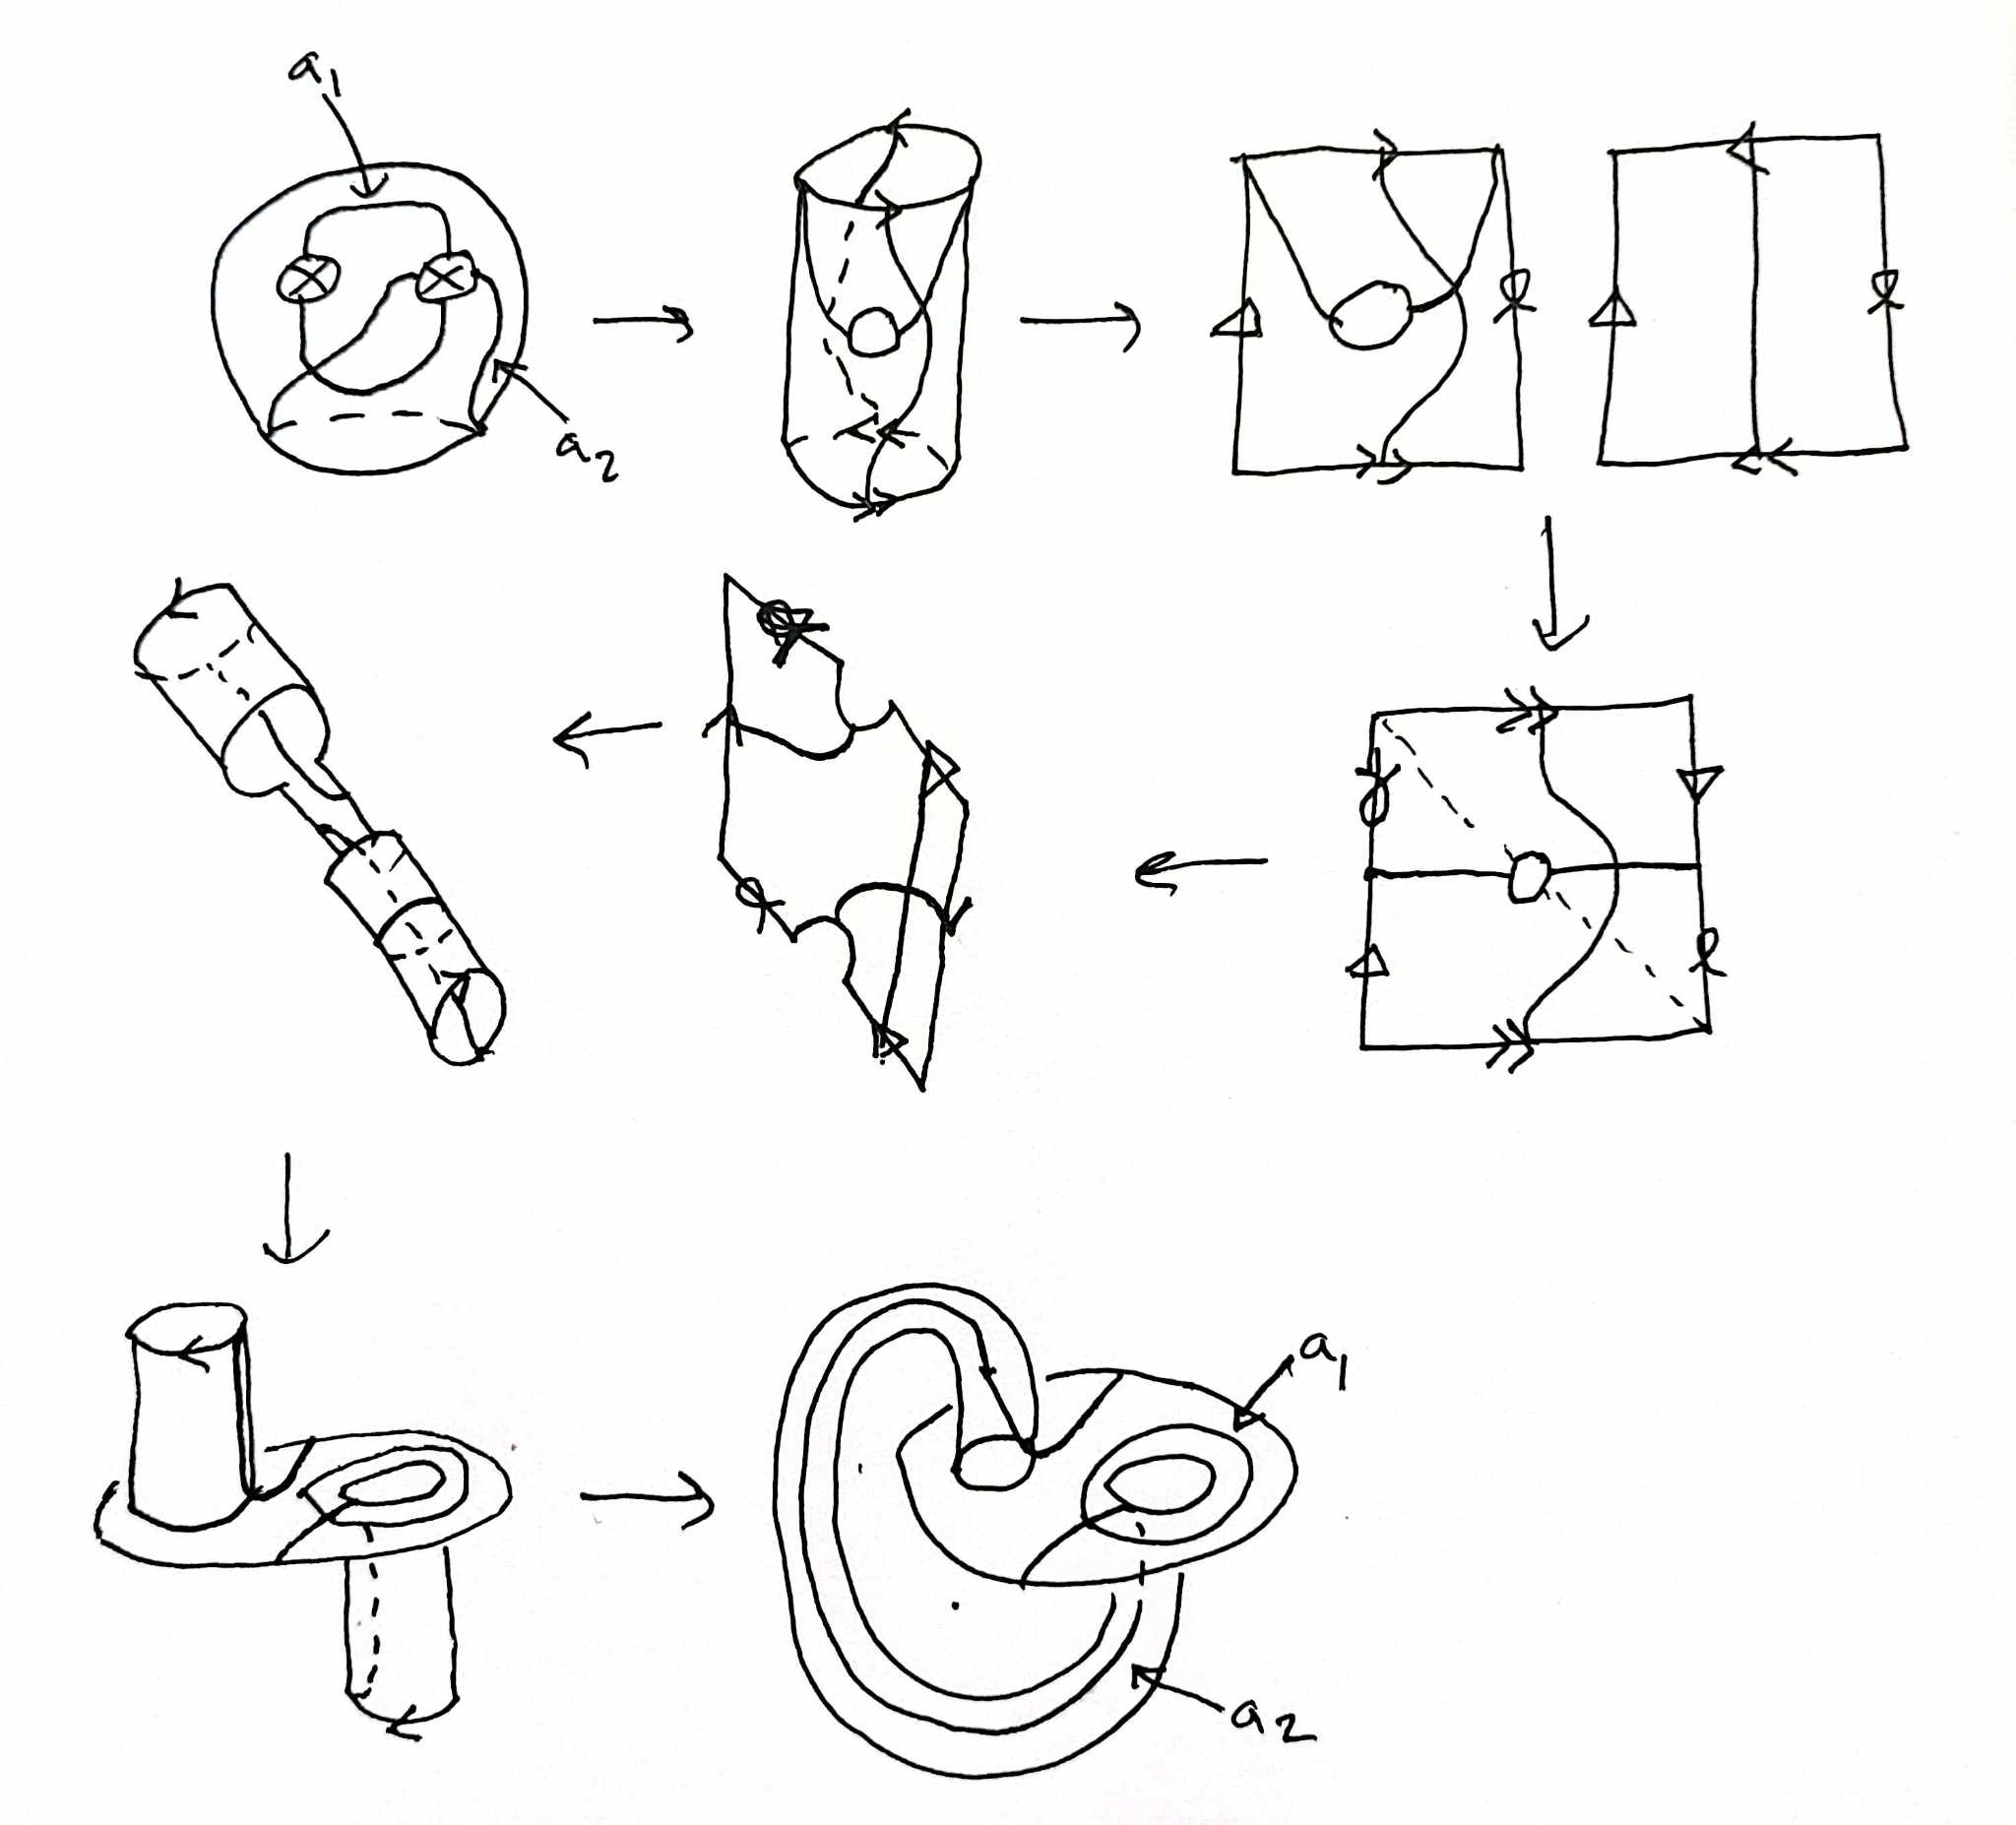
\includegraphics[width=0.8\textwidth]{part1-deformation-curve.jpg}
    \caption{The loop
    $a_1$ and the arc $a_2$ throughout the homeomorphisms for
$K-D^2$}
    \label{fig:part1-deformation-curve-jpg}
\end{figure}

\begin{figure}[htpb]
    \centering
    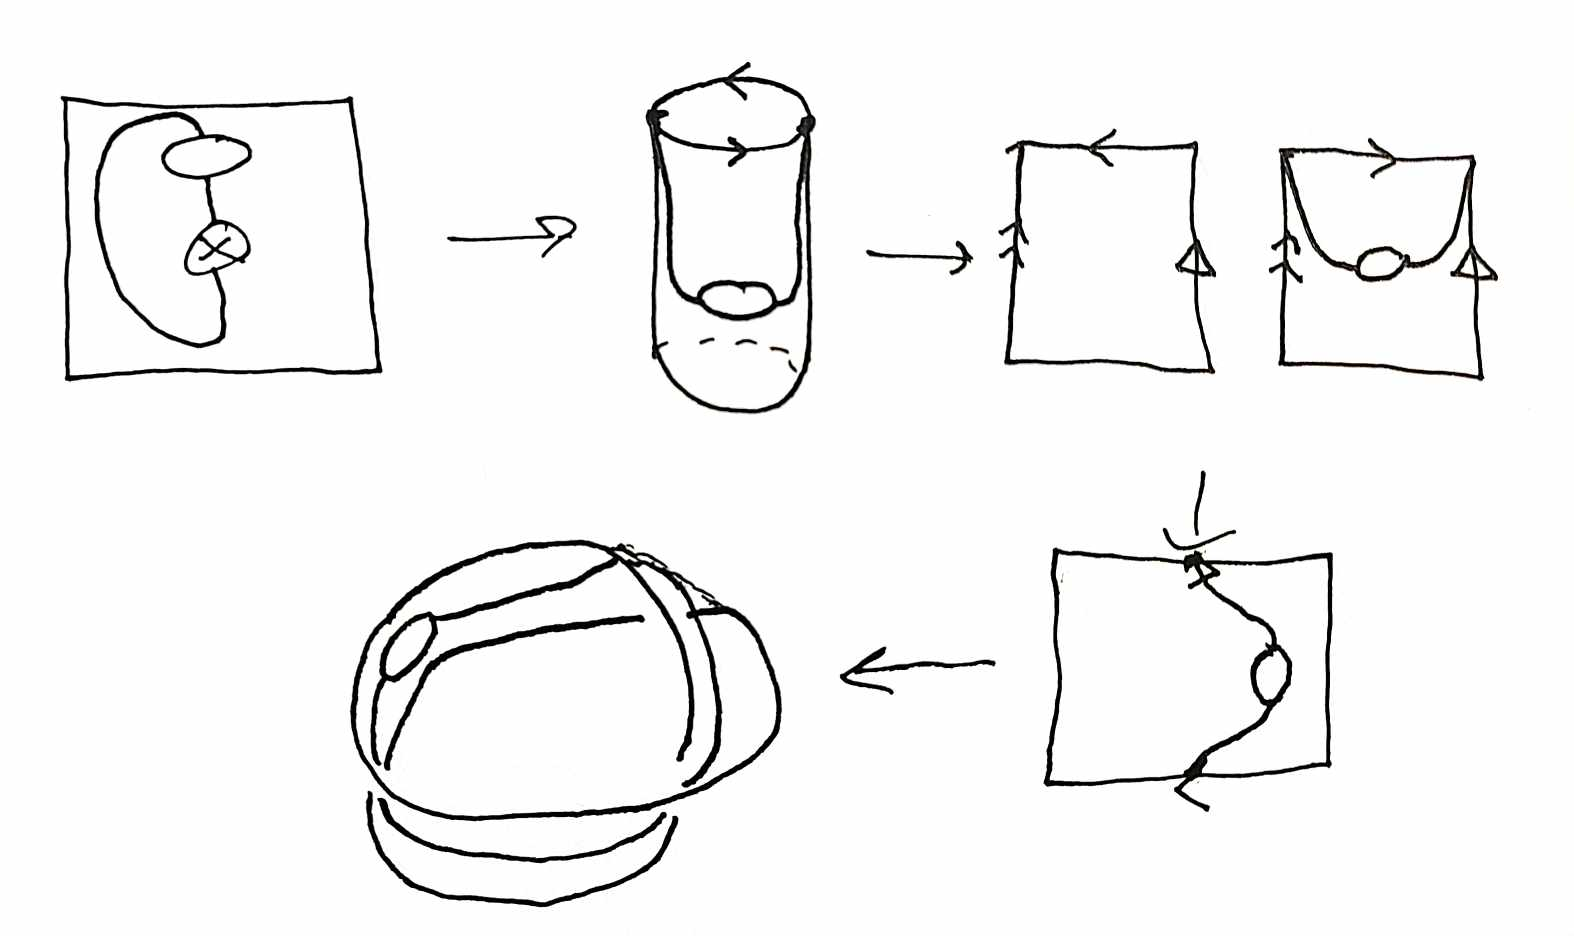
\includegraphics[width=0.8\textwidth]{part2-deformation-curve.jpg}
    \caption{The arc from $a_2$ throughout the homeomorphisms
    for $M-D^2$}
    \label{fig:part2-deformation-curve-jpg}
\end{figure}

\begin{figure}[htpb]
    \centering
    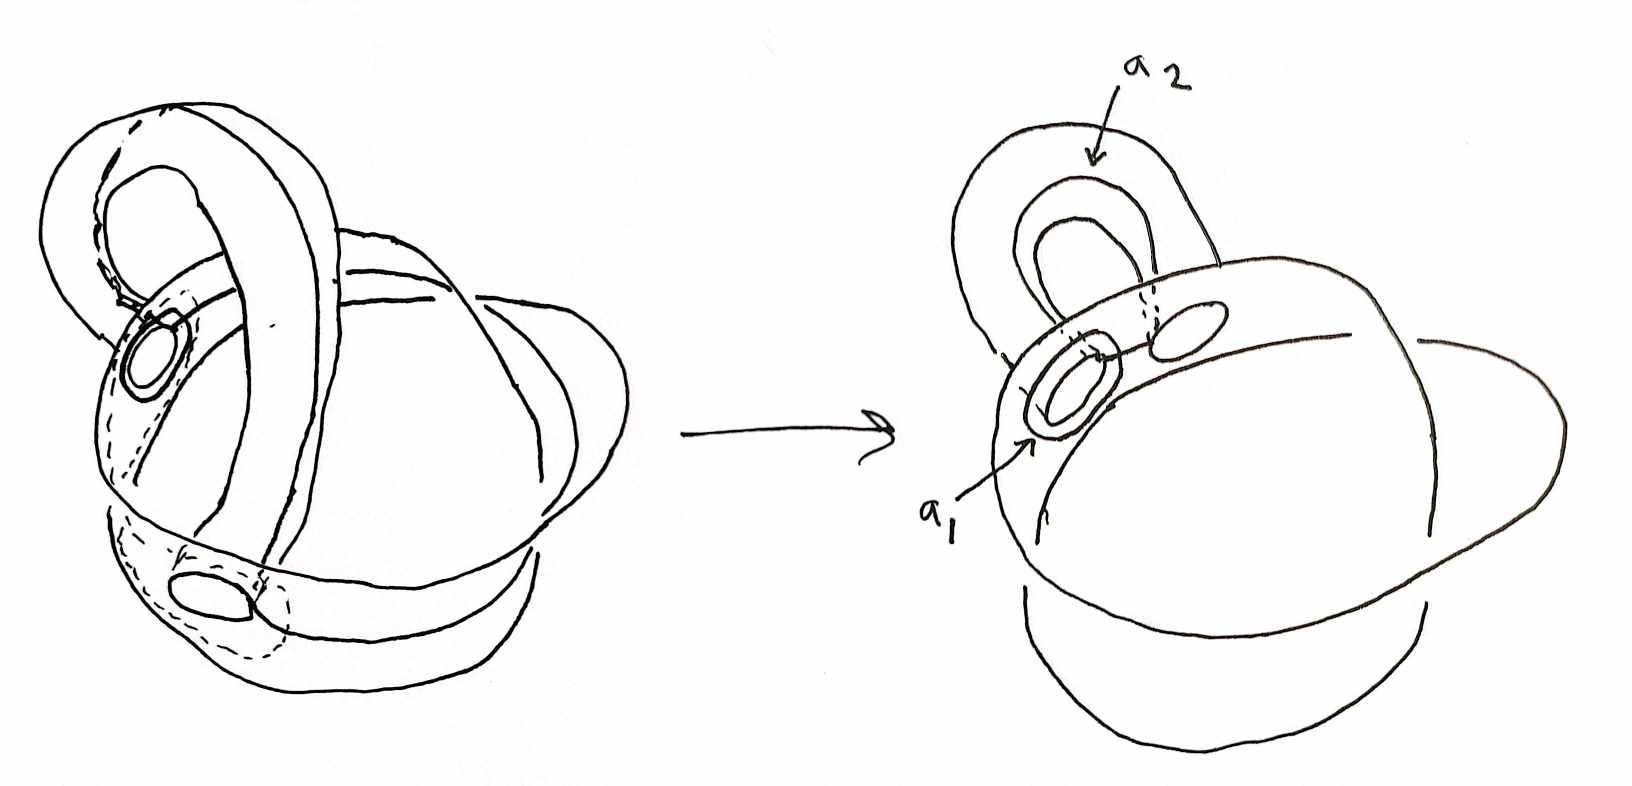
\includegraphics[width=0.8\textwidth]{klein-to-torus-curve.jpg}
    \caption{The connected sum
    of $K$ and $M$ by regluing.}
    \label{fig:klein-to-torus-curve-jpg}
\end{figure}

\begin{figure}[htpb]
    \centering
    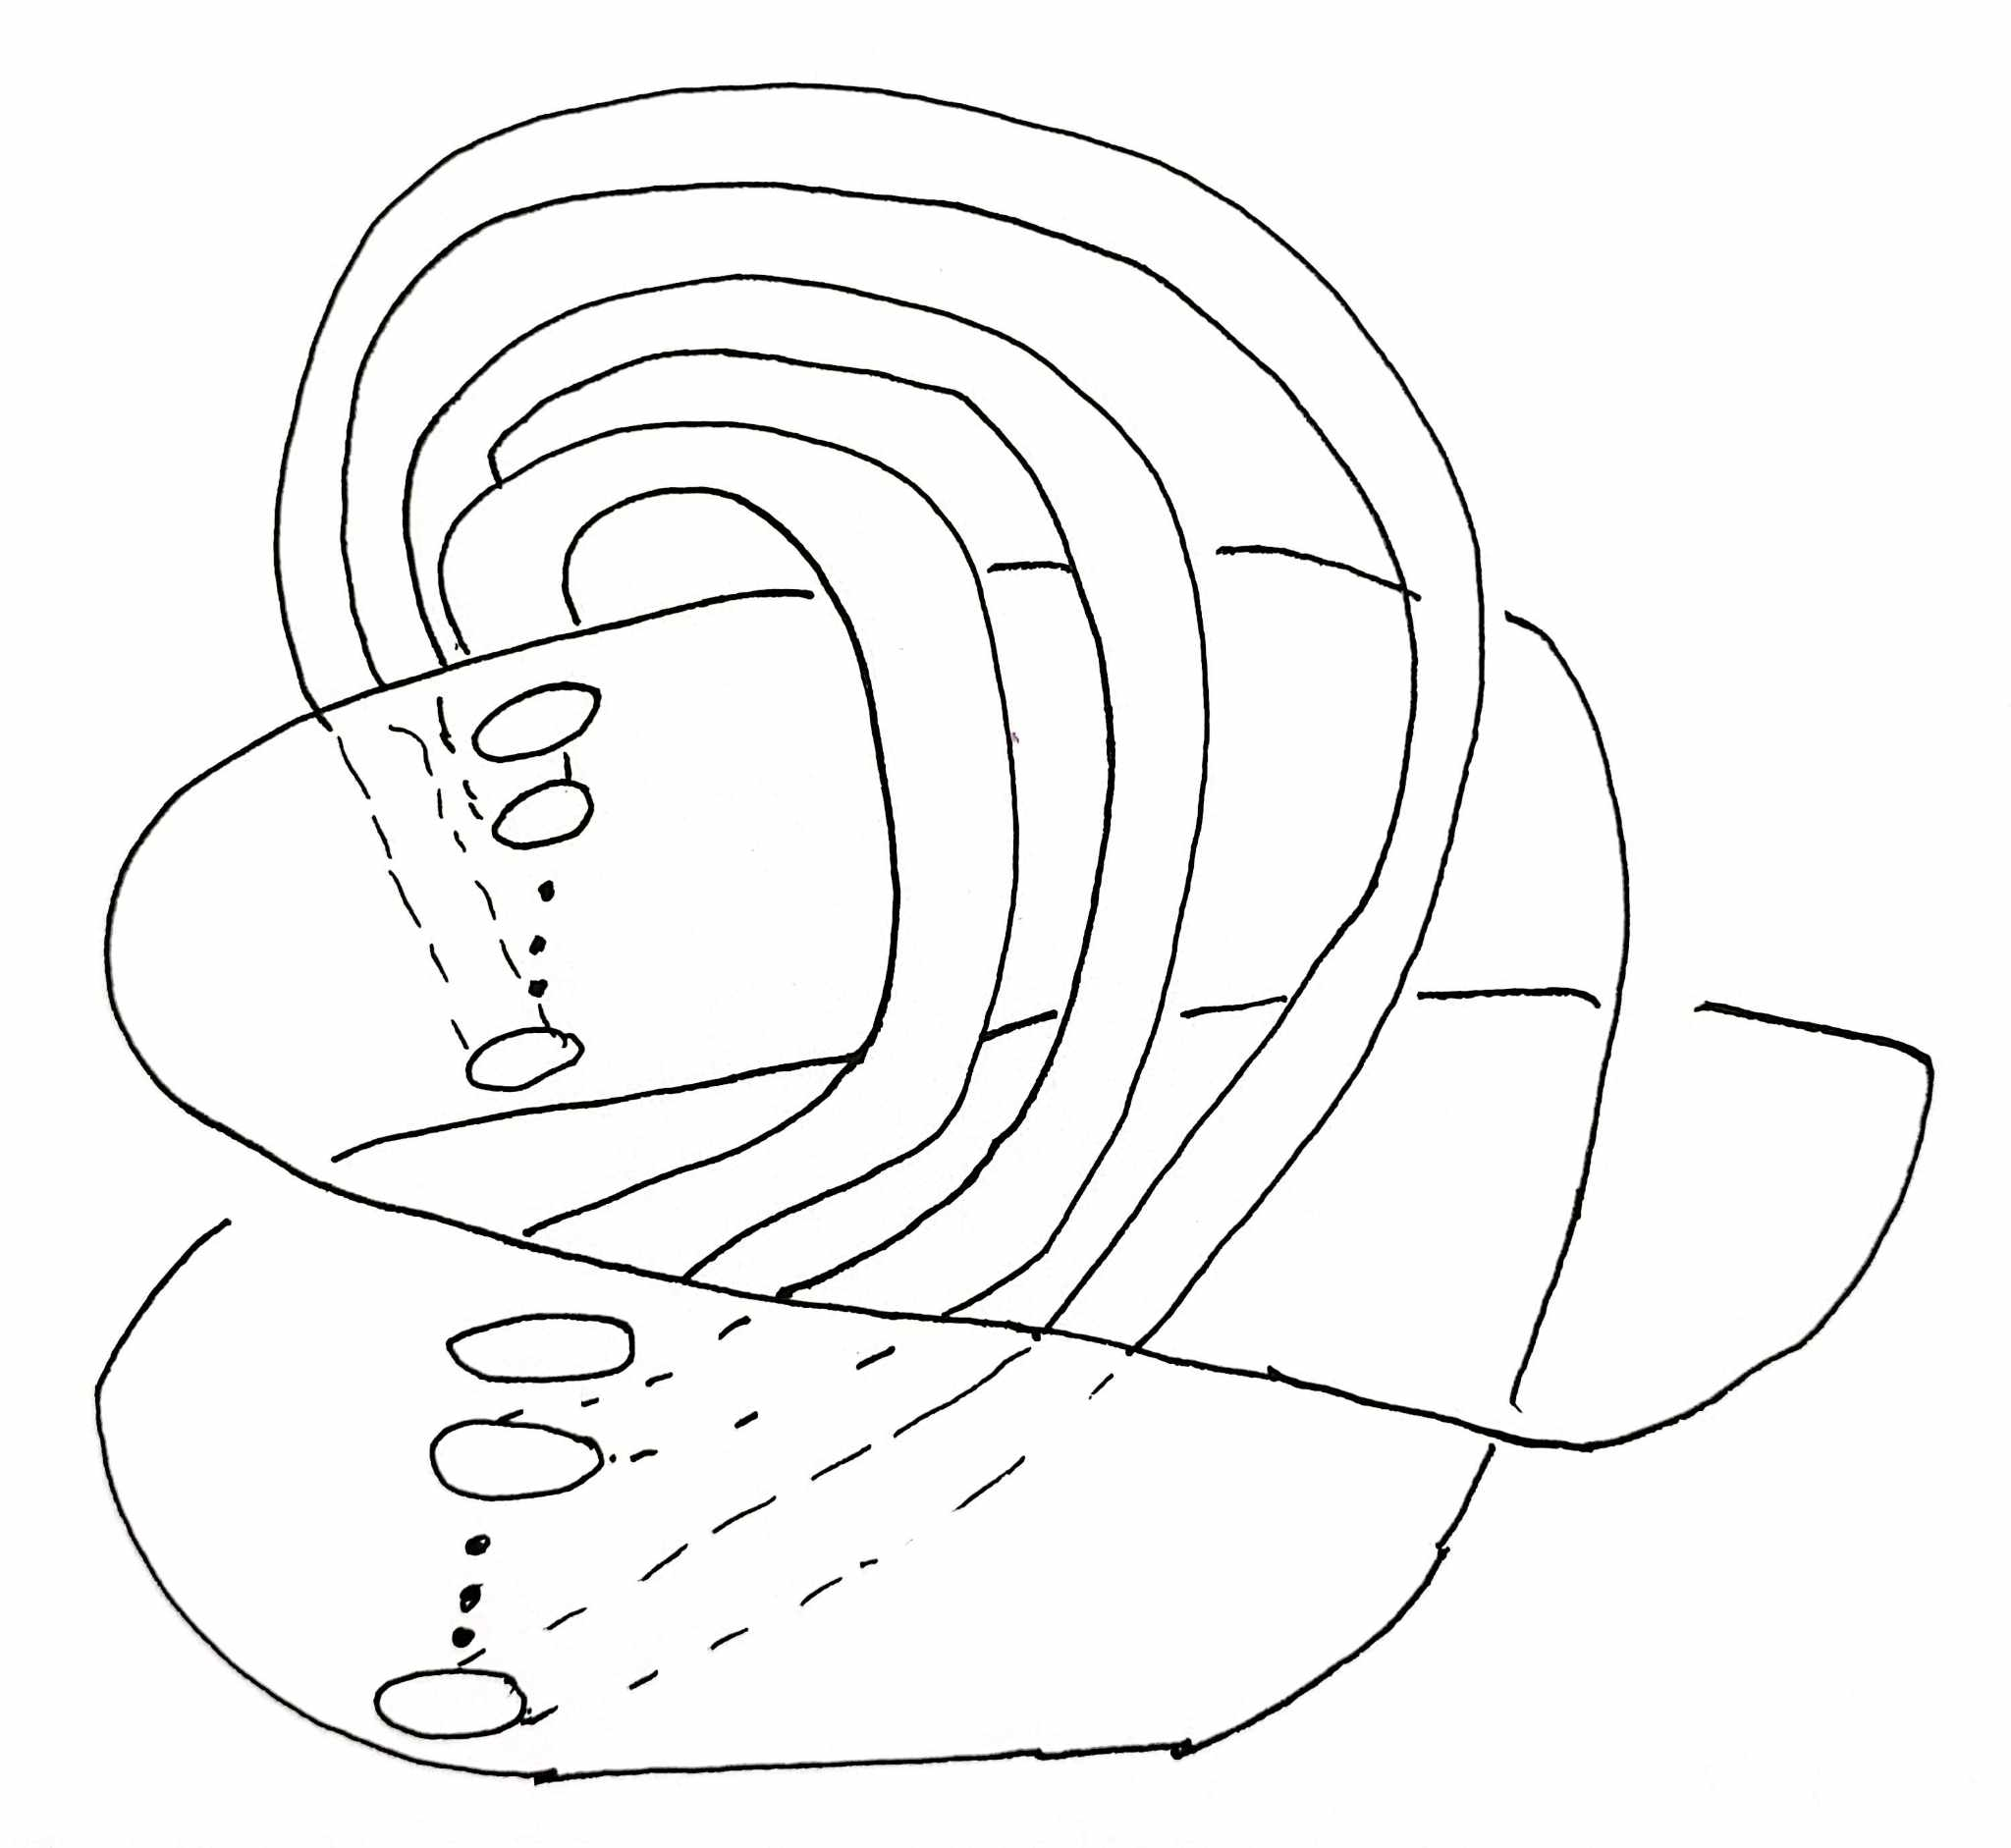
\includegraphics[width=0.5\textwidth]{many-klein-torus-curve.jpg}
    \caption{The case of $K^{\natural g} \natural M$}
    \label{fig:many-klein-torus-curve-jpg}
\end{figure}

\end{proof}

\begin{note}
    In the case where we do not have boundary components, we
    can simple remove a disk, perform the operations 
    from Proposition \ref{standard-twist-birman-hilden} and then
    reglue. Thus we can actually extend the proposition
    to the case of $b = 0$ as well.
\end{note}

\begin{question}
    What happens in the case where
    $g$ is even?
\end{question}

\begin{question}
    If $g$ is odd and $g \ge 5$, the standard chain
    can be extended by adding a curve
    $a_g$ passing once through each of the first
    $g-1$ crosscaps. This
    extended chain also determines
    a standard twist representation
    $\rho_{C'} \colon \mathcal{B}_{g+1} \to 
    \PMod \left( N_{g,b} \right) $. Does it correspond to
    something we know as well?
\end{question}

\subsubsection{The crosscap transposition representation}

Let $N = N_{g,b}$ be nonorientable. A sequence
$C = \left( a_1, \ldots, a_{n-1} \right) $ of separating
curves in $N$ is called \textit{a chain of separating curves} if
\begin{enumerate}
    \item $a_i$ bounds a one-holed Klein bottle
        for $i = 1, \ldots, n-1$,
    \item $i \left( a_i, a_{i+1} \right) = 2$ for
        $i = 1,\ldots, n-2$,
    \item $i\left( a_i, a_j \right) = 0$ for
        $\left| i-j \right| > 1$.
\end{enumerate}


Here $a_i$ bounding a one-holed Klein bottle means
that if we collapse $a_i$ to a point, we obtain a 
sphere with two crosscaps which is equivalent to the Klein bottle


Let $K_i$ be the one-holed Klein bottle bounded by
$a_i$. Then $K_i \cap K_{i+1}$ will be a Möbius strip
for $i = 1, \ldots, n-2$, and we denote its core curve
by $\mu_{i+1}$. Let $\mu_1$ and $\mu_n$ be the core curves
of $K_1 - K_2$ and $K_{n-1} - K_{n-2}$, respectively.
Fix an orientation of a regular neighborhood of
the union of the $a_i$. Let $T_{a_i}$ be the right-handed
Dehn twist about $a_i$and let $u_i$ be the 
\textit{crosscap transpostion} supported
in $K_i$, swapping $\mu_i$ and $\mu_{i+1}$ such that
$u_i^2 = T_{a_i}$ (essentially a half-Dehn twist but for crosscaps
instead of punctures).

\begin{figure}[H]
    \centering
    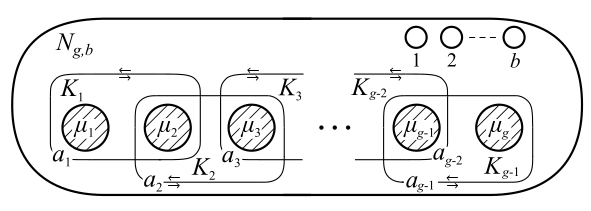
\includegraphics[width=0.6\textwidth]{chain-separating-curves.png}
    \caption{A chain of separating curves in
    $N_{g,b}$. \cite[Figure 2]{StSz}}
    \label{fig:chain-separating-curves-png}
\end{figure}


\begin{lemma}[]
    The mapping $\theta_{C} \colon B_n \to \PMod (N)$ by
    $\theta_C \left( \sigma_i \right) =u_i$ for
    $i = 1,\ldots, n-1$, defines a homomorphisms
    called crosscap transposition representation.
\end{lemma}

\begin{remark}[]
    This is simply the geometric representation
    arising from the Yang-Baxter element associated to
    the Möbius band in $\mathcal{M}_1$ which
    is the half-twist on crosscaps.
\end{remark}


\subsubsection{Transvection}

\begin{definition}[Transvection]
    Given a homomorphism
    $\rho \colon B_n \to \PMod (S)$ and an element
    $\tau \in \PMod (S)$ such that
    $\tau$ commutes with $\rho\left( \sigma_i \right) $ 
    for $1 \le i \le n-1$, we define a homomorphism
    $\rho^{\tau} \colon B_n \to \Mod (S)$, called
    a \textit{transvection} of $\rho$, by
    \[
        \rho^{\tau} \left( \sigma_i \right) 
        = \tau \rho \left( \sigma_i \right) , \quad
        i = 1,\ldots, n-1.
    \] 
    A homomorphism $\rho \colon B_n \to \PMod (S)$ is called
    \textit{cyclic} if $\rho \left( B_n \right) $ is a 
    cyclic group. 
\end{definition}

\begin{note}
    Note that transvection defines an
    equivalence relation on
    the set of representations
    $B_n \to \PMod(S)$.
\end{note}


\subsection{The main theorems}

Following work by Castel and generalizations by
Chen and Mukherjea on classifications
of geometric representations of the braid
group on orientable surfaces in certain ranges,
Stukow and Szepietowski
proved the following two theorems in \cite{StSz} which classify
all geometric representations on non-orientable surfaces
in a certain range. 

\begin{theorem}[]\label{Thm1.2}
    Let $n \ge 14$ and let $N = N_{g,b}$ with
    $g \le 2 \left\lfloor \frac{n}{2} \right\rfloor +1$ and
    $b\ge 0$. Then any homomorphism
    $\rho \colon B_n \to \PMod (N)$ is either
    cyclic, or is a transvection of a standard twist
    representation, or is a transvection of a crosscap
    transposition representation.
\end{theorem}

\begin{theorem}[]\label{Thm1.3}
    Theorem~\ref{Thm1.2} still holds
    when $\PMod (N)$ is replaced by $\Mod \left( N,
    \partial N \right) $.
\end{theorem}

Note that $\Mod (N, \partial N) \not \le 
\PMod (N)$ as, for example, the Dehn twist about a boundary
curve is non-trivial in $\Mod \left( N, \partial N \right) $, but
becomes trivial in $\PMod (N)$.\\
\linebreak
We have shown that
the standard twist representation for odd genus and the
crosscap transposition naturally arise as
Yang-Baxter operators on appropriate objects in
an appropriate category of surfaces.

By Theorem \ref{Thm1.2}, these are in fact all the possible
explicit
geometric representations which we can look at
on non-orientable surfaces
up to transvection given in
\cite{StSz}. 



          




\newpage

\printbibliography
\end{document}
